% (c) 2020 Stefan Antonowicz
% Based off of tex found at https://github.com/ludus-leonis/nipajin
% This file is released under Creative Commons Attribution-NonCommercial-ShareAlike 4.0 International License.
% Please do not apply other licenses one-way.

\renewcommand{\yggMonsters}{%
  \mychapter{The Monsters}{monsters}
    \begin{center}
    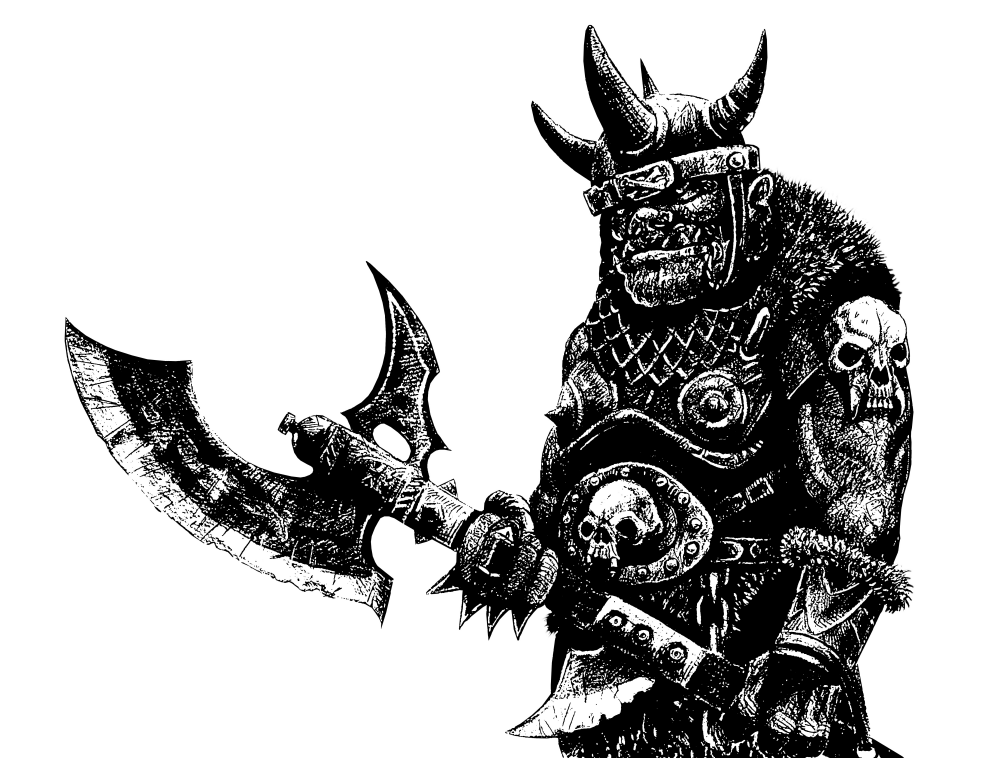
\includegraphics[width=\linewidth,keepaspectratio=true]{monsters/MonstersHeader}
    \end{center}
    \newpage
}

\renewcommand{\yggMonstersText}{%

Lurking in crypts, creeping across the moors, hiding in ruins, populating sewers - \mylink{Monsters}{roles-monster} threaten danger and death to unwary Adventurers.  The role of the Monster falls to the \mylink{The Arbiter}{roles-arbiter} to play.

\ed {
    Generally speaking, the Arbiter does little rolling for Monsters; Init, Fighting, and Guarding against their attacks falls to the Adventurer. The goal here is to give the Arbiter space to narrate what's happening in combat instead of getting bogged down with rolling dice and consulting lots of charts. 

}



    \myimage{monsters/Water_2}


    \mysubsection{Reading the Monster Block}{monster-block}


    \MONSTER[]


\mysubsection{Base Monster Stats}{monster-basic-stats}

\mytable{Y Y Y Y Y}{
    \thead{\small{{\color{toyblu}HIT}}} & \thead{\small{Damage}} & \thead{\small{Weak.}} & \thead{\small{Save}} & \thead{\small{Spells\Dagger}} \\ 
}{
    0\Asterisk & d4 & d24 & 12 & 0 \\
    1 & d6 & d24 & 11 & d4 \\
    2 & d8 & d20 & 10 & 2d4 \\
    3 & d10 & d20 & 9 & 3d4 \\
    4 & 2d6 & d16 & 8 & 3d4 \\
    5 & d6+d8 & d16 & 7 & 4d4 \\
    6 & 2d8 & d12 & 6 & 4d4 \\
    7 & d20 & d10 & 5 & 5d4 \\
    8 & d10+d12 & d8 & 4 & 5d4 \\
    9 & d24+d3 & d4 & 3 & 6d4 \\
}

\footnotesize 
\Asterisk The Monster has 1 Health 

\Dagger Magic using Monsters only
\normalsize

\mysubsection{Hit Dice}{monster-hit-dice}

\HD correspond to Adventurer Levels: a 1 \HD monster should be a match for a Level 1 Adventurer.  The higher the \HD, the greater the damage, saves, and spell dice - and the lower the Weakness.

\mysubsection{Damage}{monster-damage}

The die to roll to determine how much damage is inflicted on an Adventurer who has missed their \mylink{Guarding}{combat-guarding} try. Monsters can neither Crit nor Fumble.

\mysubsection{Weakness (WK)}{monster-weakness}

When an Adventurer makes an \mylink{Attack}{combat-attack} try, they must \RO the Monster's Weakness along with their Weapon Trait, and add their \LVL. 

Similarly, when an Adventurer makes a \mylink{Guarding}{combat-guarding} try, they must \RO the Monster's Weakness along with their \DEX, and add their \LVL.

\mysubsection{Saves}{monster-saves}

There is only one Save for a Monster that covers Hexes, Toxins, and Doom. Roll 2d6 for a Save try. If the number is greater than or equal to the Save, the Monster is successful. 
 
\mysubsection{Spell Dice}{monster-spell-dice}

Some Monsters are able to invoke Arcana-like effects. The number of Spell Dice indicate the number of d4 a Monster may use to perform their magic. Additional information can be found in the \mylink{Spells}{monster-spells} section below.

\mysubsection{Health (Hlth)}{monster-health}

Health indicates the amount of damage the Monster can take before it dies. Health is a function of \mylink{Hit Dice}{monster-hit-dice} times \mylink{Power}{monster-power}: Weak creatures have 3 Health per \HD; Average creatures have 5 Health per \HD; and Strong creatures have 7 Health per \HD. 

\mysubsection{Speed (SPD)}{monster-speed}

When an Adventurer tries \mylink{Init}{combat-init}, they must \RO using the Monster's Speed along with their \INT and \MD.

Monster Speed also indicates which die to roll in a \RB{\DEX} contest.

\mytable{l X X X}{
    \thead{} & \thead{Slow} & \thead{Base} & \thead{Fast}  \\
}{
    Speed & d20 & d16 & d12 \\
    \DEX & d6 & d8 & d10 \\
}

\mysubsection{Power}{monster-power}

Power measures how many points of Health a Monster has per \HD, and which die to roll if a \VIG \RB is required:

\mytable{l X X X}{
    \thead{} & \thead{Weak} & \thead{Average} & \thead{Strong}  \\
}{
    Health & 3 per HIT & 5 per HIT & 7 per HIT \\
    \VIG & d6 & d8 & d10 \\
}

\mysubsection{Attack (ATK)}{monster-attack}

Attack indicates the number of targets a Monster can attack ("1 Close" or "6 Nearby", for instance). Attacks against multiple targets are listed as one of three types, listed in the Monster's description:

\mybullet {
    \item \mybold{Combined} means that the multiple attacks can only target a \mybold{single} Adventurer i.e. the Adventurer will have to roll their Guard multiple times to avoid getting hurt.
    \item \mybold{Distinct} means that the multiple attacks can only target \mybold{multiple} Adventurers i.e. each Adventurer only has to roll their Guard once.
    \item \mybold{Either} means that the multiple attacks can either be Combined or Distinct, at your discretion.
}


\mysubsection{Soak}{monster-soak}

Soak is a Monster's \mylink{Armor}{gear-armor}, representing thick scales, tough or rubbery bodies, etc.  Like Armor, the Soak die is rolled whenever \mybold{physical} damage is taken, and the damage is reduced by that amount. A roll of 1 or 2 on the Soak die means the die moves \DCDOWN (just like Armor). Certain Monsters may only have Soak against specific types of weapons (for example, Skeletons have d4 Soak vs. Stabbing damage).  \mylink{Murder}{vulgate-whispers-murder} bypasses Soak. Most Monsters have a Soak of 0.

  \mytable{l X}{
    \thead{Soak} & \thead{Examples}  \\
  }{
    d4 & Armored troops, Skeletons, etc. \\
    d6 & Knights, Giant Beetles, etc. \\
    d8 & Automatons, Powerful Demons etc. \\
    d10 & Dragons, Titans, etc.   \\
  }

\end{multicols*}
\newpage

\myimage{monsters/MonsterCreation}

\begin{multicols*}{2}
   \mysubsection{Morale}{monster-morale}

Morale measures the likelihood of a Monster running away when things go against them.  Roll 2d6 for a Morale try. If the number is greater than or equal to the basic roll, the Monster attempt to flee or surrender. If a Monster turns tail and runs, any Adventurer Close to it may attempt an Attack try \myital{before} the Monster moves to the next range hex, provided they still have Actions left this Moment.

\mysubsection{Traits and Actions}{monster-traits-and-actions}

Monster \mylink{Monster Traits}{monster-traits} and \mylink{Innate Abilities}{monster-innate} are dealt with in the appropriate section below.


\cbreak

Monsters are Cowardly, Orderly, or Fanatical:



\callout{\footnotesize{
\mybullet {
  \item \mybold{Cowardly} Basic roll is 4.  If the Monsters are in a group, roll a) when the first Monster dies (but only if the Monsters are outnumbered; b) when half the Monsters are down; or c) whenever a "leader" dies.  If the Monster is by itself, roll a) when it first takes damage and b) when it's at half Health or less.

  \item \mybold{Orderly} Basic roll is 8.  If the Monsters are in a group, roll a) when half the Monsters are down; or b) if \mybold{all}  the leaders are dead.  If the Monster is by itself, roll when it's at half Health or less.

  \item \mybold{Fanatical}  Basic roll is 12.  If the Monsters are in a group, roll when half the Monsters are down AND all the leaders are dead.  If the Monster is by itself, it will automatically pass a morale check.
}}}







\newpage

  

\mysection{Spells}{monster-spells}

Monstrous spell-casters roll one or more \UDD{d4} to perform their magic. Monstrous spell-casters do not suffer any ill effects from rolling triples, quadruples, or quintuples. 

Roll a d8 to see what their "basic" spell is, or choose from the list below. 


\myimage{monsters/Flavor_6}

\mybold{1. Bomb}
The Monster manifests a storm of frogs / ice storm / fireball / blast of seawater, etc. somewhere Close, Nearby, or Far Away.  Everyone Close to the manifestation takes \SUM+\DICE damage (Save for half), plus an incidental effect (things catch fire, fires are doused, etc.).

\mybold{2. Boost}
The Monster yells a rallying cry / summons the spirits of the ancestors / asks the Fates for a boon, etc. that can either grant a Monster a +\DICE bonus on damage or inflict a -\DICE \RO or \RS penalty on an Adventurer (Save negates).

\mybold{3. Fix}
The Monster is a mechanical genius / has healing saliva / restores the faith of the injured, etc. and can repair, heal, etc. \SUM+\DICE Health on themselves or another Monster.

\mybold{4. Shoot}
The Monster throws a magic dart / spits a viscous glob / shoots beams from its fingers / yells a word like a knife, etc. at an Adventurer Nearby, Far-Away, or Distant.  The projectile doesn't miss and deals \SUM+\DICE damage. 

\mybold{5. Stun}
The Monster breathes out a somnolent gust / lets out a stunning shriek / paralyzes with a look, etc. against \DICE Adventurers either Close or Nearby.  If the Adventurer fails their Save, they are slept / stunned / paralyzed for a duration depending on the number of dice spent:

  \mytable{c X c} {
    \thead{\DICE}  & \thead{} & \thead{\Duration} \\
  } {
    1 & & d4  \\
    2 & & d6 \\
    3 & & d8 \\
    4 & & d10 \\
    5 & & d12 \\
    6+ & & d16 \\
  }


\mybold{6. Aspect}
The Monster gains giant lobster claws / sticky hands like a fly / a hundred spider eyes, etc. for \SUM Moments.  The effect depends on the trait but should grant a +\DICE bonus (to damage, \RS checks, etc.).

\mybold{7. Armor}
The Monster summons a whirlwind of butterflies / a shield of shrieking shadows / the ability to blink in and out of existence, etc.  They gain \SUM points of protection - treat this as if it were extra Health, subtracting from this amount first.

\mybold{8. Summon}
The Monster summons \DICE Zoological / Elemental / Demonic creature(s) whose total \HD do not exceed \DICE (see the section on \mypg{the Obliterated}{forgotten-obliterated} for details.


  \newpage
  \mysection{Orders}{monster-orders}

Monsters are categorized into various Orders, each with one or more Traits.  The Traits are common to all the species beneath the Order.

In addition to these Orders are two specific Genera - \mypg{Dragons}{monster-dragons} and \mypg{Elementals}{monster-elementals} - that are dealt with separately.

\cbreak

% MONSTER ORDER BEGIN
\MONSTERORDER{Aberrations}{monster-order-aberrations}{Alien - Canny}

Monsters that come from "outer space" or other dimensions, or Monsters created in a lab by fucked-up Philosophers.


\MONSTERORDER{Amphibians}{monster-order-amphibians}{Slippery - Zoological}

Toads, salamanders, troglodytes and other cold-blooded Monsters found in or around bodies of water.  

\MONSTERORDER{Arthropods}{monster-order-arthropods}{Venomous - Zoological}

Giant spiders, beetles, and other insects.

\MONSTERORDER{Automatons}{monster-order-automatons}{Mindless - Unhallowed}

Golems, robots, and living statues usually created by Mystics who subsequently lost control of them.


\MONSTERORDER{Demons}{monster-order-demons}{Chaotic - Otherworldly - Terrifying - Unhallowed}

Perversions of the will of \TheAuthority and residents of \mybold{Limbo}. Demons are cunning, intelligent, charismatic, and thoroughly and unapologetically fucking evil.


\MONSTERORDER{Dinosaurs}{monster-order-dinosaurs}{Frenzied - Terrifying - Zoological}

Big-ass, pants-shitting thunder lizards.  



\MONSTERORDER{Dire Beasts}{monster-order-dire-beasts}{Berserk - Zoological}

Large "Ice Age" types of mammals.


\MONSTERORDER{Giantkin}{monster-order-giantkin}{Strong - Stupid}

\myimage{monsters/GiantTopper}

Massive bipedal creatures known for both their extraordinary strength, ferocity, and breathtaking stupidity.


\MONSTERORDER{Goblinoids}{monster-order-goblinoids}{Canny - Nocturnal}

Cousins of Giantkin but comparatively smaller.  What they lack in size and strength they make up in cunning.  Goblinoids can't stand direct sunlight.


\MONSTERORDER{Goos}{monster-order-goos}{Amorphous - Mindless - Splitting}

Various slimes, jellies, and molds that are sentient(?) and hell-bent on killing Adventurers.



\myimage{monsters/Goo_1}

\MONSTERORDER{Horrors}{monster-order-horrors}{Nocturnal - Terrifying - Unhallowed}

Ghouls, ghasts, lycanthropes, and liches - soulless Monsters that strike fear into the hearts of mortals.



\MONSTERORDER{Plantlife}{monster-order-plantlife}{Pack - Supportive}

Sentient plants and intelligent fungus.   Plantlife seem to be able to communicate with one another in a way that's almost telekinetic.



\MONSTERORDER{Reptiles}{monster-order-reptiles}{Frenzied - Zoological}

Cold-blooded, air breathing Monsters like snakes and lizards.  If you're looking for dragons, they get their \mylink{own section}{monster-dragons}.



\MONSTERORDER{Shades}{monster-order-shades}{Otherworldly - Spectral - Terrifying - Unhallowed}

Ghosts, spirits, vampires, and restless spectres.  

\cbreak

\MONSTERORDER{Swarms}{monster-order-swarms}{Mindless - Swarming - Zoological}

Plagues of rats, swarms of locusts, or crawling blankets of scorpions.



\myimage{monsters/Horrors_2}

\MONSTERORDER{Walking Dead}{monster-order-walking-dead}{Dead - Mindless - Unhallowed}

Corporeal creatures risen from the grave.  




% MONSTER ORDER END

  \newpage
  \mysection{Traits}{monster-traits}

Monsters have specific Traits associated with them that gives them a little extra "juice" when it comes to killing Adventurers.  Some of these Traits are common to the entire \mylink{Order}{monster-orders} that the Monster belongs to, while other Traits are specific to the Monster.  

% MONSTER TRAITS BEGIN
\mysubsection{Acidic}{monster-trait-acidic}

\mybullet {
  \item Acidic Monsters remove 1 \UD of Armor whenever they successfully deal damage.
  \item Acidic Monsters release an acrid plume of smoke when slain.  The smoke causes coughing and choking for 1 Minute to everything Nearby (-2 to \RO and \RS tries) unless a \SAVE{Toxins} is made.
}

\mysubsection{Alien}{monster-trait-alien}

\mybullet {
  \item Alien Monsters are immune to \mylink{Toxins}{malignants-toxins}.
  \item Alien Monsters are immune to \mylink{Secrets of Biomancy}{arcana-wizardry-secrets}.
}

\mysubsection{Amorphous}{monster-trait-amorphous}

\mybullet {
  \item Amorphous Monsters are immune to \mylink{Murder}{vulgate-whispers-murder} (no definable anatomy).
  \item Amorphous Monsters can slip through cracks under doors, ooze up walls, hang on ceilings, etc.
}

\mysubsection{Amphibious}{monster-trait-amphibious}

\mybullet {
  \item Amphibious Monsters can breathe in water and on land.
}

\mysubsection{Berserk}{monster-trait-berserk}

\mybullet {
  \item Berserk Monsters will fight until the bottom of the \myital{next} Moment after they are reduced to 0 Health.
}

\mysubsection{Bloodthirsty}{monster-trait-bloodthirsty}

\mybullet {
  \item Bloodthirsty Monsters can smell blood.
  \item Bloodthirsty Monsters will concentrate their attacks on Adventurers who have taken Flesh damage.
}

\myimage{monsters/Imp}

\mysubsection{Cannibal}{monster-trait-cannibal}

\mybullet {
  \item In lieu of attacking, Cannibalistic Monsters can spend their turn consuming part of a corpse to heal 3 Health.
}

\mysubsection{Canny}{monster-trait-canny}

\mybullet {
  \item Canny Monsters are clever - they strategize, coordinate, set traps, and ambush.
}

\mysubsection{Chaotic}{monster-trait-chaotic}

\mybullet {
  \item Chaotic Monsters are immune to \mybold{all} Arcana except the \mylink{Secrets of Entropy}{arcana-wizardry-secrets}.
  \item Chaotic Monsters are \mylink{Unhallowed}{monster-trait-unhallowed}.
}

\mysubsection{Dead}{monster-trait-dead}

\mybullet {
  \item Dead Monsters are immune to \mylink{Toxins}{malignants-toxins}.
  \item Dead Monsters speak \mylink{Graveborn}{idiolect-graveborn}.
}

\mysubsection{Elemental}{monster-trait-elemental}

\mybullet {
  \item Elemental Monsters immune to \mybold{all} Arcana except the \mylink{Secrets of Elements}{arcana-wizardry-secrets}.
}


\mysubsection{Flying}{monster-trait-flying}

\mybullet {
  \item Flying Monsters can spend an Action moving one range step (Close to Nearby, Nearby to Far-Away, etc.) up or down, adding an additional dimension to their movement.
}

\mysubsection{Frenzied}{monster-trait-frenzied}

\mybullet {
  \item Frenzied Monsters do +1 damage for every Moment after the first (cumulative).
}

\mysubsection{Leaping}{monster-trait-leaping}

\mybullet {
  \item Leaping Monsters can jump up to 10m forward, backward, or upward. 
  \item If a Leaping Monster jumps into Combat, treat their attack as a \mylink{Charge}{monster-action-charge}.
}

\myimage{monsters/Flavor_3}


\mysubsection{Militant}{monster-trait-militant}

\mybullet {
  \item Militant Monsters get a +2 on their Morale rolls.
  \item Militant Monsters will cooperate and act tactically.
}

\mysubsection{Mindless}{monster-trait-mindless}

\mybullet {
  \item Mindless Monsters are immune to \mylink{Secrets of the Mind}{arcana-wizardry-secrets}.
  \item Mindless Monsters have no morale (they fight until they die).
}


\mysubsection{Nocturnal}{monster-trait-nocturnal}

\mybullet {
  \item Nocturnal Monsters can see in the dark.
  \item Adventurers gain a +4 bonus to \RO and \RB tries against Nocturnal Monsters if the Monster is in direct sunlight.
}

\mysubsection{Otherworldly}{monster-trait-otherworldly}

\mybullet {
  \item Otherworldly Monsters are immune to damage from iron weapons.
}

\mysubsection{Pack}{monster-trait-pack}

\mybullet {
  \item Pack Monsters deal +1 damage for every other Pack Monster who is Close to them.
}

\mysubsection{Slippery}{monster-trait-slippery}

\mybullet {
  \item Slippery Monsters cannot be \mylink{Grappled}{combat-deeds-grapple}.
  \item Slippery Monsters take 0 damage from \mylink{Unarmed attacks}{combat-damage-unarmed}.
}

\mysubsection{Spectral}{monster-trait-spectral}

\mybullet {
  \item Spectral Monsters can pass through doors and walls.
}



\mysubsection{Splitting}{monster-trait-splitting}

\mybullet {
  \item Splitting Monsters split in half if they take 7+ damage in a single attack.  These new Monsters have half of the Monster's current Health, rounded up, after the damage is applied.
}


\mysubsection{Strong}{monster-trait-strong}

\mybullet {
  \item Strong Monsters can perform feats of strength (break through chains, pick up anvils, etc.) at the Arbiter's discretion.
}

\mysubsection{Stupid}{monster-trait-stupid}

\mybullet {
  \item Stupid Monsters are easily tricked and do not strategize.
}

\mysubsection{Supportive}{monster-trait-supportive}

\mybullet {
  \item Supportive Monsters can heal \HD Health on any Close Monster of the same species (but not themselves).
}

\mysubsection{Swarming}{monster-trait-swarming}

\mybullet {
  \item Swarming Monsters can attack all targets Close to them during their Action.
  \item Swarming Monsters share their Health as one pool.
  \item Swarming Monsters are not affected by Stabbing weapons.
}


\mysubsection{Terrifying}{monster-trait-terrifying}

\mybullet {
  \item Terrifying Monsters require an \INSANITY try when an Adventurer encounters them for the \mybold{first} time.
}

\cbreak

\mysubsection{Twitchy}{monster-trait-twitchy}

\mybullet {
  \item Twitchy Monsters always win Init (Pooka still beat them though).
}


\myimage{monsters/Giant_2}


\mysubsection{Unhallowed}{monster-trait-unhallowed}

\mybullet {
  \item Unhallowed Monsters have no soul.  
  \item Unhallowed Monsters are affected by Curse the Unhallowed.
  \item Unhallowed Monsters cannot enter Hallowed Ground.
}

\mysubsection{Venomous}{monster-trait-venomous}

\mybullet {
  \item Venomous Monsters deliver an \mylink{Noxious Toxin (d6)}{malignants-toxins} if they strike Flesh. \SAVE{Toxins} negates.
}

\mysubsection{Zoological}{monster-trait-zoological}

\mybullet {
  \item Zoological Monsters are considered "Beasts" for the purposes of summoning, etc.
}

% MONSTER TRAITS END

  \newpage
  % (c) 2020 Stefan Antonowicz
% Based off of tex found at https://github.com/ludus-leonis/nipajin
% This file is released under Creative Commons Attribution-NonCommercial-ShareAlike 4.0 International License.
% Please do not apply other licenses one-way.

\renewcommand{\yggCombat}{%
  \mychapter{Combat}{combat}
  \mysectionheader{combat/CombatHeader}
  \newpage
}

\renewcommand{\yggCombatText}{%

    \mysection{Fighting}{combat-fighting}

  \callout {
  \mybullet {
    \item Combat is conflict that takes place between \mybold{Adventurers} and \mybold{Monsters} at a particular \mybold{Distance}.

    \item Combat consists of \mybold{Moments} and takes \mybold{Minutes} to complete. 

    \item Each Moment you make an \mybold{Init} try to determine how many Actions you get.  If you \RO, you get 2 Actions; otherwise, you get 1 Action.

    \item If you have 2 Actions, you can take 1 \mybold{before} the Monsters' turn and one \mybold{after} the Monsters' turn. If you have 1 Action, you can only take it \mybold{after} the Monsters' turn.

    \item There are 2 kinds of Actions: Maneuver Actions and Combat Actions. When you take a Combat Action, your Moment ends.

    \item Certain Actions occur at the Top or Bottom of the Moment.
  }}

  See the section on \mypg{the Game}{the-game} for more info on these terms.



  \mysubsection{Who Goes First?}{combat-init}

  \mybold{The Init try} decides whether your Adventurer will take 1 or 2 Actions this Moment. 

Before the Init try is rolled, the Arbiter must determine if one side (your Band, or the Monsters) got \mybold{the Drop} on the other.

\myimage{combat/Fighting1}

\cbreak



  \mysubsection{The Drop}{combat-drop}

  You sneak up on a couple of ogres arguing over who gets to eat which half of Dwight the Unlucky, or you come around the corner right into an ambush. The Arbiter will first determine if either side gains the \effect{Surprised}. If the Arbiter determines that you've Surprised the Monster, you get \mybold{the Drop} on them (and if you are Surprised, the Monsters have gotten the Drop on you!).

  If the Monsters get the Drop on you, they get to act for a full Moment before you roll your Init. Any damage you take before you make your Init try \mybold{bypasses Grit}. If you get the Drop on the Monsters, you get to act for a full Moment before they do. Any damage you deal to the Monsters are \mybold{Crits} (see "Dealing Damage" below).

Additionally, if you have a \mylink{Knave}{trope-knave} or \mylink{Murk}{species-murk} in your Band, the Drop allows them to attempt a \mybold{Murder} by using their knowledge of the Whispers of the Bride (see the section on \mypg{Whispers}{vulgate-whispers} for more details).


    Once the Drop is resolved, all Allies must try their \mybold{Init} at the top of the Moment. If you successfully \RO, you can take 2 Actions (1 \myital{before} the Monsters take their turn, and one \myital{after}); if you aren't able to assemble a 20 in this \RO try, you go \myital{after} the Monsters take their turn. The Init try is your \INT plus your \mylink{Movement Die}{combat-movement-die} plus the \mypg{Monster's Speed}{combat-monster-speed}.


  \formula{Init Try}{
    \RO: \INT \PLUS \MD \PLUS \mybold{Monster Speed}
  } 


\newpage

  \myhighlight{The Movement Die}{combat-movement-die} \MD

  \mylink{Armor}{gear-armor} is great to have if you plan on getting hit, but it has a cost - the heavier and more cumbersome the Armor, the lower your Move Die. Each type of armor has a \MD associated with it:

  \mytable{Y Y}{
    \thead{\mylink{Armor}{gear-armor}} & \thead{\MD} \\
  }{
    None & d20 \\
    Light & d12 \\
    Medium & d8 \\
    Heavy & d4  \\
  }


  \myhighlight{The Monster's Speed}{combat-monster-speed}

  Most Monsters you meet are going to have a speed of d16. Some Monsters are Fast - their speed is d12.  Some Monsters are Slow - their speed is d20.  See the section on \mypg{Monsters}{monsters} for more details.

  \myimage{combat/Combat_1}


\cbreak

  \crunch{Mixed Init}{combat-mixed-init}

  If the Allies are fighting Monsters with mixed speeds (a group of slow blood puppets led by a necromancer who moves at normal speed, say), use Init as follows:



\callout{\footnotesize{
  \mynumlist {
    \item  The Allies roll their Init against the necromancer (d16 speed).  If they \RO, they can take an Action (see below).
    \item  The necromancer takes her turn.
    \item  Any Allies that won Init against the necromancer can take their second Action now.  Any Allies who failed to \RO against the necromancer should now test their Init against the blood puppets.  If they \RO, they can take an Action.
    \item  The blood puppets take their turn.
    \item  Allies who have any Actions left, or Allies who failed both Init tests now take their Action.
  }
}}

\newpage

\end{multicols*}
  \mysubsection{Actions}{combat-actions}

  Combat consists of \mybold{Moments} and takes \mybold{Minutes} to finish. Each Moment you make an Init try to determine how many Actions you get.  If you \RO, you get 2 Actions; otherwise, you get 1 Action.

  If you have 2 Actions, you can take 1 Action \mybold{before} the Monster and 1 Action \mybold{after} the Monster. If you fail, you can only take 1 Action \mybold{after} the Monster. You can always choose to act after - there's no need to roll at that point. You can act as a group and decide your own order for Actions in each Moment. 

  Your Action can be either a \mybold{Maneuver} or \mybold{Combat} Action. Maneuver Actions (Basic and Tactical) cover you moving around the battlefield, attending to hurt Allies, getting things out of your pack, setting up attacks, etc. Combat Actions (Deeds and Attacks) are actions taken to actually fight with a Monster. You can only take 1 Combat Action every Moment - taking a Combat Action immediately ends your turn.


  \myctrtable{Y Y}{
    \thead{Maneuver Actions} & \thead{Combat Actions} \\
  }{
    Basic & Deed \\
    Tactical & Attack \\
  }


\vspace{2pt}

\begin{multicols*}{2}

  \mysubsection{Maneuver Actions}{combat-maneuvers}

  \callout {
    Getting better position, pulling something from your pack, etc. Maneuver Actions are divided into \mybold{Basic} and \mybold{Tactical} Maneuvers. Taking a Maneuver Action does \mybold{not} end your Moment.
  }

  \myhighlight{Basic Maneuver}{combat-basic-maneuver}

  Basic Maneuvers involve positioning yourself in combat, readying equipment, picking up something you dropped, etc.  A Basic Maneuver is anything that might take you a handful of seconds to do.  For example:

  \mybullet { 
    \item Move somewhere Nearby;  
    \item Ready a shield and/or weapon; 
    \item Switch weapons; 
    \item Pick up something you dropped; 
    \item Get up from the Prone position; 
    \item Light a torch or flaming oil; 
    \item Grab something out of your pack; 
    \item Drink a potion or applying a salve;
    \item etc.
  }

  Whether or not something qualifies as a Basic Maneuver is up to the Arbiter's discretion.  It's possible that a Basic Maneuver might take multiple Actions. Some examples:

  \mybullet {
    \item Picking a lock while a fight rages around you;
    \item Tying off a rope and swinging into combat;
    \item Running across the room to dig through a fallen Ally's pack;
    \item Trying to find a spell inside a Grimoire;
    \item etc.
  }

  The Arbiter should decide how many Actions this will take ("it'll take you a Basic Maneuver to tie off the rope and another Basic Maneuver to swing into Combat"; "it's a Basic Maneuver to move Nearby, another Basic Maneuver to roll him over and open his pack, and a third Basic Maneuver to find that salve of wound binding").

\end{multicols*}
  \myhighlight{Tactical Maneuver}{combat-tactical-maneuver}

  Tactical Maneuvers utilize the environment of the battlefield to positively influence Combat. You can only use one Tactical Maneuver at a time, and you can't "stack" them (you can't \mybold{Aim} for multiple Moments and stack the bonuses, for instance). Unless it says otherwise, bonuses and penalties apply to the next \RO check.


\begin{multicols*}{2}


  \COMBAT [
    Name = Aim,
    Link = combat-tactical-maneuver-aim,
    Desc = Shoot or Throw Weapons Only
  ]
  
  You take careful aim with your weapon.  If your \myital{next} Attack \RO hits, you \mybold{Crit} (you still must roll your \FOC). The benefit lasts until you take a Combat Action or something breaks your aim (moving, taking damaging, Guarding, etc).

  \COMBAT [
    Name = Block,
    Link = combat-tactical-maneuver-block,
    Desc = Brawl weapons only
  ]

  Get in a Monster's way and try to get it to attack you.  You can either "pick a fight" with a Monster Close to you, or move somewhere Nearby and get in the way. Try your \RSTRY{\PRE}.  If you succeed, the Monster will attack you at its next opportunity.

  \COMBAT [
    Name = Brace,
    Link = combat-tactical-maneuver-brace,
    Desc = Polearm or spear only
  ]

  Set your polearm or spear to defend against incoming Monsters.  If a Monster \mypg{Charges}{monster-action-charge} (including Leaping) during its Action, you may immediately take a Combat Action \mybold{before} the Monster attacks (provided you haven't taken a Combat Action already).

\cbreak

  \COMBAT [
    Name = Rage,
    Link = combat-tactical-maneuver-rage,
    Desc = Brawl weapons only
  ]

  You take an Action to gain \effect{Enraged}.  The target of the rage is "the Monsters". If one of your Allies has injured you in this fight, they count as a Monster.

  \COMBAT [
    Name = Reckless,
    Link = combat-tactical-maneuver-reckless,
    Desc = Brawl weapons only
  ]

  You use an Action to aggressively position yourself against the Monsters.  You gain a bonus modifier to your next Attack \RO and a double penalty to your next Guard \RO i.e. take +2 to Attack but -4 to Guard.  You can only gain up to +4/-8 in this way.

  \COMBAT [
    Name = Warding,
    Link = combat-tactical-maneuver-warding,
    Desc = Brawl weapons only
  ]


  You use an Action to defensively position yourself against the Monster.  You gain a bonus modifier to your next Guard \RO and a double penalty to your next Attack \RO i.e. take +2 to Guard but -4 to Attack. You can only gain up to +4/-8 in this way.

\begin{figure*}
\begin{center}
\myimage{combat/CombatShieldWall}
\end{center}
\end{figure*}


\newpage


  \mysubsection{Combat Actions}{combat-combat-actions}

  \callout {
    You commit to your attack and take a Combat Action. Combat Actions are divided into \mybold{Deed} and \mybold{Attack} Actions. Taking a Combat Action \myital{immediately} ends your turn in this Moment.
  }


  \myhighlight{Deeds}{combat-deeds}

  Deeds cover special kinds of attacks you might try to make. You can only use one Deed at a time (you can't use Bum Rush and Florentine at the same time, for example); unless it says otherwise, bonuses and penalties apply to the next \RO check. Deeds are Combat Actions, and taking a Combat Action ends your Moment.

  \COMBAT [
    Name = Bash,
    Link = combat-deeds-bash,
    Desc = Must have a shield equipped (it has to be on your arm / you have to be using it)
  ]

  Get the Monster's attention.  Make an Attack try, but deal damage as if you were \mylink{Unarmed}{combat-damage-unarmed}. If you hit, the Monster will attack you at the next opportunity.


  \COMBAT [
    Name = Bum Rush,
    Link = combat-deeds-bum-rush,
    Desc = Must be attacking with a \VIG Brawl weapon
  ]

  Charge!  Move somewhere Nearby and immediately make an Attack try.

  \COMBAT [
    Name = Disarm,
    Link = combat-deeds-disarm,
    Desc = Brawl weapons only. Your target must be using a 1-handed weapon
  ]

  Make an Attack try.  If your try succeeds, make a \RBONE{\VIG} or \RBONE{\DEX} (your choice) vs. your opponent's \VIG or \DEX (Arbiter's choice). If you win you deal no damage, but your opponent is \effect{Disarmed}.


  \COMBAT [
    Name = Florentine,
    Link = combat-deeds-florentine,
    Desc = Must be attacking with two Daggers\, two Shortswords\, or a mix of both
  ]

  Make an Attack try. If you hit, roll damage for both weapons and pick the highest:

  \mylist {
    \item  If both dice are natural 1s, you automatically Fumble.
    \item  If one die is a natural 1, the other die can't Crit (even if you roll \MAX damage).
  }

  \COMBAT [
    Name = Gambit,
    Link = combat-deeds-gambit,
    Desc = Arbiter gets to add penalties to your roll depending on how crazy it is.
  ]

  Called shot. Make an Attack try, but roll twice.  If both hit, it happens.  If one hits, it doesn't.  If neither hit, you automatically Fumble.

  \COMBAT [
    Name = Grapple,
    Link = combat-deeds-grapple,
    Desc = You must be either unarmored or in Light Armor
  ]

  Make an Attack try. If you succeed, the Monster is grappled. You and the Monster are both considered \effect{Prone} until the grapple is broken, meaning Attack and Guard Actions against the Monster get a +4 bonus. However, if an attack against the Monster misses, \RSTRY{\DEX} - a Failure means you are forced to release the Grapple. 

 At the top of the Moment, make an \RB using your \VIG or \DEX (your choice) vs. the Monster's \mypg{Power}{monster-power} or \mypg{Speed}{monster-speed} (Arbiter's choice). If you ever lose the \RB try or take any damage, the grapple is broken.

 Only one Adventurer can grapple a Monster at a time.

  \COMBAT [
    Name = Sunder Shield,
    Link = combat-deeds-sunder,
    Desc = Must have a shield equipped (it has to be on your arm / you have to be using it)
  ]

  If a Monster's attack is about to cause you \mybold{physical} damage, you may immediately destroy your shield, taking no damage. You can wait until after the damage is rolled to decide if you're sundering your shield.  If you already took a Combat Action this Moment, you can't use this Deed.


  \myimage{combat/Combat_2}


  \myhighlight{Attacks}{combat-attack-action}

  \formula{Attack Try}{
    \RO : Weapon Trait \PLUS Monster Weakness \PLUS your Level 
  }

  Eventually your maneuvering and mighty deeds of arms will manifest into a strike at your opponent. The Attack action is when you roll your dice to see if you are able to hit the Monster you're in combat with.

  To see if you hit a Monster, \RO using your weapon's \mypg{Trait}{gear-weapons} plus the Monster's \mylink{Weakness}{monster-weakness}, and add your \LVL to the result. If you fall short, you can try to Bump your result above a 19 by rolling various other dice (a Sellsword's \mypg{Prowess}{sellsword-prowess}, the associated die of your \mypg{Personality}{adventurer-personality}, etc.).

  If you succeed in your Attack try, you deal damage to the Monster.

\end{multicols*}

  \mysubsection{Dealing Damage}{combat-dealing-damage}

  The damage your weapon does is a single die. Weapon damage is found in the section on Weapons under \mypg{Gear}{gear}.  You roll the die and deal that much damage to the Monster.  If you roll a 1, you might Fumble.  If you roll \MAX damage on the die, you might Crit.



  \myhighlight{Crits and Fumbles}{combat-crits-and-fumbles}

  If you roll \MAX damage, your blow may be a Crit. Make a \RSTRY{\FOC} try.  If you roll a Failure, nothing happens. Otherwise, add +4 to your damage.

  If you roll a natural 1 for damage, your blow may be a Fumble. Make a \RSTRY{\FOC} try. If you roll a Failure, you deal no damage to the enemy, and must roll on the table below. The die you use is specified by your \mylink{Armor's}{gear-armor} weight.

  \myctrtable{Y Y}{
    \thead{Weight} & \thead{Die}  \\
  }{
    None & d2  \\
    Light & d4  \\
    Medium & d8 \\
    Heavy & d12 \\  
    Shield & +1 to roll \\
    Helmet & +1 to roll 
  }



If something doesn't apply, move up the chart (that is, things get worse) to the next available effect that works.

\callout{\footnotesize{
\mynumlist {
  \item You miss spectacularly and everyone laughs at you and now no one will invite you to prom.  Lose 1 Grit on account of the shame.
  \item You miss and lose your grip on your weapon and you're holding it all awkward and things feel weird.  Your next Attack try is -4.
  \item You tell everyone that your opponent dodged but really you got all turned around.  Your next Guarding try is -4.
  \item You trip and fall - you are now \effect{Prone}.
  \item You \effect{Disarm} yourself. If it's a Shoot weapon, the bowstring breaks and it'll take Minutes to fix, so let's hope you have a plan B.
  \item If you're wearing a backpack you sever the straps, it splits open, and all the contents spill onto the ground.  Backpack is now useless and everyone can see your weird collection of things you've been stealing.
  \item You really overextend yourself, pull a hammy, and mess up your \mylink{Armor}{gear-armor} (if you're wearing any).  Make an Armor \UD roll.
  \item (or more) Stop hitting yourself!  The damage bypasses your Grit and applies to you instead.
}}}

\newpage
\begin{multicols*}{2}

\myhighlight{Lethal Damage}{combat-damage-lethal}

Certain mighty warriors and terrifying Monsters deal \mybold{Lethal} damage. If they roll \MAX damage, they roll again, adding the second roll to the first. If they roll the \MAX again, they repeat the process. Continue rolling until you do not roll \MAX. Modifiers to damage are added or subtracted \mybold{after} the die explodes (from rolling \mylink{Prowess}{sellsword-prowess}, for instance).

    \example{Charse the Lethal attacks a goblin with a Shortsword (d6).  He rolls his Attack try and hits, and rolls a 6 for damage. He rolls again and rolls another 6.  He rolls a 3rd time and rolls a 4.  He deals 16 points of damage(!) (6+6+4) and the goblin is reduced to a fine pink mist.}


\cbreak

  \myhighlight{Unarmed Damage}{combat-damage-unarmed}

  Your damage for Unarmed combat depends on your \VIG

  \mytable{Y Y}{
    \thead{\VIG} & \thead{Damage} \\
  }{
    d6 & 1  \\
    d8 & 2  \\
    d10 & 3  \\
    etc.
  }

  If you bring someone to 0 Flesh via Unarmed combat, they are \effect{Knocked Out} for \DUR{d4}.  Continued Unarmed attacks against Knocked Out foes prompt \DEATH rolls as you beat them to death.

  Note that since this isn't a die roll there's no way to Crit or Fumble.  Fighting unarmed is the same as using a weapon with the \VIG Trait.



  \newpage
  \mysection{Guarding}{combat-guarding}

  \flavor{Go that way, really fast. If something gets in your way, turn. \\~ \Tilde Charles de Mar, \myital{Better Off Dead}}


  It is generally considered a \myital{really good idea} to avoid getting struck by claws, swords, and falling debris. Guarding is when you roll your dice to see if you are able to avoid getting hit by the Monster you're in combat with.

  \formula{Guarding Try}{
    \RO : Your \DEX \PLUS Monster Weakness \PLUS Your \LVL
  }



  To see if you can dodge the Monster, you must \RO with a Guarding try.  To make a Guarding try, roll your \DEX with the Monster's \mylink{Weakness}{monster-weakness}, and add your \LVL to the result. If you fall short, you can try to bump your die roll above a 19 by rolling various other dice (the Sellsword's \mylink{Prowess}{sellsword-prowess}, the associated die of your \mylink{Personality}{adventurer-personality}, etc.)

  If you fail in your Guarding try, you take damage from the Monster.

  \myhighlight{Taking Damage}{combat-taking-damage}

  Taking damage works in roughly the same way as dealing damage, except the Arbiter rolls for Monster damage.  \mybold{Monsters cannot Crit or Fumble}. The Arbiter is encouraged to roll the damage out in the open. The \SUM of the damage is applied to your Adventurer Sheet in the order specified to the right.

\cbreak

\begin{center}
  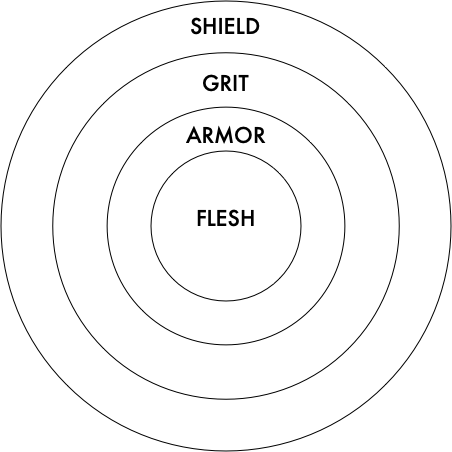
\includegraphics{combat/THE_ORDER}
\end{center}

  \mynumlist {
    \item \mybold{Shield} : If you have a shield equipped (that is, on your arm) and take \mybold{physical damage}, and you haven't taken a Combat Action yet, you can \mylink{Sunder}{combat-deeds-sunder} your shield. Stop here.  Otherwise ...
    \item \mybold{Grit} : Subtract the damage from your Grit.  If there's any damage left over, move to Armor i.e. if I have a Grit of 4 and I take 9 damage, I have 5 damage left over and I move on to Armor.
    \item \mybold{Armor} : If you have armor, see how much damage it will absorb.  Roll the \UD for your armor and subtract the result from the damage.  For example, if I'm wearing chain mail (Medium armor) I roll a d8; if I rolled a 5, I'd subtract 5 from the total damage. If I roll a Failure with my Armor, I still subtract the damage, but move the \UD \DCDOWN. If there's any damage left over, move onto Flesh.
    \item \mybold{Flesh} : Subtract the rest of the damage from Flesh. If you go to 0 or less Flesh, you are \mylink{Dying}{combat-dying}.
  }

  \newpage
   \mysection{Dying}{combat-dying}

 \mybold{If your Flesh ever goes to 0 or below, you are Dying}.  


Your Grit immediately drops to 0 (if it isn't 0 already), and your Flesh is set to 0. Grit can't be healed if you're Dying, only Flesh.

  While at 0 Flesh you can't do anything but crawl to safety and hold your intestines in. If you do \myital{anything} more strenuous than this, make a \DEATH try. \mybold{If you roll a Failure, you immediately perish}. Continue trying your \DEATH at the top of every Moment you continue to do anything more than lie there. 

  If you continue to take damage (you're \mylink{Bleeding}{effect-bleeding}, someone continues to beat on you as you crawl to safety, etc.) you must make a \DEATH try for \myital{each} point of damage you take i.e. if you're Dying and you take 5 damage, you must succeed on 5 \DEATH tries.  Good luck!

  Unless noted in their Trope or Species, all Adventurers' \DEATH starts at Precarious (d3).  Additional levels of \DEATH can be learned during \mylink{Advancement}{advancement}.

  The moment you are healed above 0 Flesh (through Resting, Leechcraft, etc) you are no longer Dying, but you must \myital{immediately}: 

\callout {
 \mybullet {
    \item Roll your \INSANITY (and apply its result), and
    \item Roll your \INJURY (and apply its result).
 }
}

\cbreak

\myimage{combat/Skull}

If your Adventurer should die, their Mortal soul journeys to \mylink{Limbo}{the-afterlife}, where it resides for seven days before departing. If your Adventurer does not have a soul when they perish - if they are Unseelie, or afflicted in some way - they immediately wink out of existence as if they never were.  See the section on \mylink{the Afterlife}{the-afterlife} (and \mylink{Katabasis}{occultism-katabasis}) for more info.




  \newpage
   \mysection{Recovering}{combat-resting}

  \mysubsection{Taking a Breather (Minutes)}{combat-resting-breather}

  Combat takes Minutes to finish, no matter how many Moments actually occurred.  Once Combat is over, you can take a \mybold{Breather}.  Restore 4 Grit up to your \MAX (unless an \mylink{Injury}{adventurer-kismet-injury} prevents you from doing so) plus whatever \mylink{Narcotics}{gear-narcotics} or \mylink{Arcana}{arcana} might restore.  If you have the Sellsword Virtue \mylink{Second Skin}{sellsword-virtue-second-skin}, you can repair a \UD of Armor as well, up to its \MAX.

  You don't need to take a Breather in a safe place, but common sense should prevail - taking a quick nap in front of the goblin horde after you beheaded the chieftain isn't OK.  You can only take 1 Breather per Combat.


  \mysubsection{Taking a Bivouac (Hours)}{combat-resting-bivouac}

  If you need a longer rest, you can set up camp and take a Bivouac. When sleeping rough in this way, there is the risk of \mylink{Wandering Monsters}{arbiter-monsters-wandering} finding you unless you take precautions. Each time you make a Bivouac, make a \UD roll of your \mylink{Personal Provisions}{gear-equipment} (you can share Personal Provisions with others, but you have to roll for each person).  If you don't have enough Personal Provisions, you can't get any of the good effects. 

  \mybold{If an \mylink{Injury}{adventurer-kismet-injury} doesn't prevent you from doing so:}

\callout {

  \mybullet {
    \item Restore 1 Flesh. 
    \item Set your Grit to \MAX. If your Grit was higher than \MAX, the beneficial effect ends.
    \item Restore 1 \UD of your \mylink{Armor}{gear-armor}, up to its \MAX.
    \item Restore 1 \UD of \myital{one} aspect of your \mylink{Personality}{adventurer-personality}, up to its \MAX.
  }
}

  \cbreak\bump

  \mybold{Additionally, where applicable:}

\callout {

  \mybullet {
    \item Restore \DCUP of your \mylink{Prowess}{sellsword-prowess}.
    \item Restore \DCUP of your Lucky Die (\mylink{Knave}{knave-lucky-die} or \mylink{Pooka}{pooka-lucky-die}).
    \item Restore \DCUP of your \mylink{Juju}{cruces-mojo-juju}.
    \item Restore \DCUP of your \mylink{Ingenuity}{cruces-knowledge-ingenuity}.
    \item Restore 2 \mylink{Blood Dice}{cruces-blood-dice}.
    \item Restore your \mylink{Grace Die}{vulgate-sacraments-grace}.
    \item Restore 1 \mylink{Sovereignty}{remembrance}.

  }

}


Note that "up to \MAX" is implied in all of the above.


\mysubsection{Taking Downtime}{combat-resting-downtime}

You may need to take Days, Weeks, or Months to repair the damage done to yourself (as well as spend your treasures!).  See the \mylink{Downtime}{downtime} section under \mylink{Settlements}{civilization-settlements} for more info on resting for Days, Weeks, or Months.

\myimage{combat/Campfire}

  \newpage



} %end

  \newpage\raggedbottom
  \end{multicols}

\mysection{Bestiary}{monster-list}


\mysubsection{Adventurers as Monsters}{player-versus-player}


You may encounter a situation where two (or more) Adventurers wish to engage in Combat with one another; alternately, you may wish to stat an Adventurer of your own, and sic them on the Band.  

Simply switch all \RO tries to \RB tries, change levels to Weakness using the \mylink{Basic Monster table}{monster-basic-stats}, and let the dice fall where they may.

\example {  El Ravager (a Sellsword) (Level 6) and Knuckles the Thief (Level 7) decide they've had enough of one another, and throw down.  El Rav's Weakness is d12 and Knuckles Weakness is d10.  Both roll their Init; El Rav rolls a 14 while Knuckles rolls a 12.  Knuckles decides to "bump" his roll by rolling his Luck die, and gets a 4 - making his roll a 16.  He goes first (though El Rav could retaliate by rolling his \TAL, for instance).

\myskip

Knuckles tries his Attack and El Rav tries his Guard.  After rolling various dice (Deed Dice, Luck Dice, Personality, etc)  Knuckles ends up with a 27 and El Rav rolls a 25.  El Rav takes the 12 damage Knuckles rolled to his Grit, then moves in for the kill ...

}

\myimage{monsters/Flavor_5}
\newpage



% MONSTERS BEGIN


\mysubsection{Aberrations}{monster-order-aberrations-detail}
\begin{multicols}{2}\raggedbottom




\MONSTER[
  NM=Otyugh,
  LK=monster-otyugh,
  SPD=Base,
  AT=2d8 1 Close AND d8 2 Nearby (Different),
  WK=d10,
  HD=7,
  PR=Average,
  SK=0,
  MR=Orderly,
  SV=5,
  SPL=0,
  TRT=\mylink{Alien}{monster-trait-alien}; \mylink{Canny}{monster-trait-canny},
  ACT=\mylink{Grapple}{monster-action-grapple}
  ]

If you're a Philosopher exploring eldritch blood magics, you're going to generate a lot of trash.  Failed experiments.  Leftover parts.  Weird glowing stones that you figure you probably shouldn't dump into the town water supply.  At some point, someone had the brilliant idea to breed something that could get rid of all that waste; sadly, he or she was probably killed by their creation before it escaped their laboratory.  Otyugh breed prolifically (the details are vague) in carrion, gong fields, and garbage pits.  It's a good idea to keep them well fed, though, lest they start to get hungry ...

The Otyugh attacks 2 Close or Nearby Adventurers with its tentacles, and 1 Close  Adventurer with its bite.  \RBTRY{\VIG}{\VIG} if you are struck with a tentacle or become Grappled.  The Otyugh bite automatically hits a Grappled Adventurer.

\myimage{monsters/Abberation}




\MONSTER[
  NM=Owl Bear,
  LK=monster-owl-bear,
  SPD=Base,
  AT=d6+d8 1 Close,
  WK=d12,
  HD=5,
  PR=Strong,
  SK=0,
  MR=Fanatical,
  SV=7,
  SPL=0,
  TRT=\mylink{Alien}{monster-trait-alien}; \mylink{Canny}{monster-trait-canny}; \mylink{Strong}{monster-trait-strong}; \mylink{Bloodthirsty}{monster-trait-bloodthirsty},
  ACT=\mylink{Rage}{monster-action-rage}
  ]
\callout{
    Owlbears roll a d12 for \VIG tries.
}
At some point some Philosopher figured that breeding an owl with a bear would be a really great idea.  They weren't entirely wrong - Owlbears make great guardians and security systems, but they're really, really bad companions and pets.  Nevertheless, Owlbear eggs are worth a great deal to Philosophers who want to train them for their own laboratories (they have about a 20\% success rate, with the other 80\% either not being viable or killing and maiming their "masters").





\MONSTER[
  NM=Priest of Syrinx,
  LK=monster-priest-of-syrinx,
  SPD=Base,
  AT=see below,
  WK=d12,
  HD=5,
  PR=Weak,
  SK=0,
  MR=Cowardly,
  SV=7,
  SPL=4d4,
  TRT=\mylink{Alien}{monster-trait-alien}; \mylink{Canny}{monster-trait-canny}; \mylink{Supportive}{monster-trait-supportive},
  ACT=None
 ]
\callout{

    Priests of Syrinx are immune to \mylink{Secrets of the Mind}{arcana-wizardry-secrets}.

    \hrulefill

    Priests of Syrinx have limited telepathy.  \mylink{Murder}{vulgate-whispers-murder}  attempts will not work on them, and they can see Invisible creatures.
}

Strange cephalopod headed creatures from some place among the stars.  They speak an alien language that no one has yet been able to decipher (possibly the key rests in the limited telepathy they appear to share).  Priests of Syrinx worship a supremely logical and utterly evil alien intelligence.

In addition to their spells, Priests of Syrinx wield Possibility Swords - blades of psionic energy that collapse possibilities to a single point.  At the top of the Moment, roll 3d6.  You may use any combination of these dice to either reduce physical damage by the amount shown on the die, or deal damage to up to 3 Close Adventurers.   The blade strikes automatically and cannot be Guarded.  

\example {
   At the top of the Moment, you roll 3d6 with a result of 6, 5, 1.  A Sellsword Adventurer wins Init and strikes, hitting for 7 points of damage.  You use the 6 to reduce this damage to 1.  On your turn, you strike back at the Adventurer for 6 (5+1) damage - you could also have split the attack between the Sellsword and one of her compatriots (5 points on one and 1 point on the other)
}

The Possibility Sword requires whatever limited telepathy the Priests of Syrinx possess in order to work correctly.


\MONSTER[
  NM=Rust Monster,
  LK=monster-rust-monster,
  SPD=Base,
  AT=d4 1 Close,
  WK=d20,
  HD=3,
  PR=Average,
  SK=d4,
  MR=Orderly,
  SV=9,
  SPL=0,
  TRT=\mylink{Alien}{monster-trait-alien}; \mylink{Canny}{monster-trait-canny},
  ACT=None
 ]
Also known as the "Philosopher's Friend", created and bred to level the playing field.  If an Adventurer with Medium or Heavy armor is struck by a Rust Monster, immediately roll the Armor's \UD \mybold{before} attempting to absorb the attack.  If a Rust Monster is struck by an iron weapon, treat the weapon's damage as a \UD (in other words, move the weapon's damage die \DCDOWN if a 1 or a 2 is rolled).


\MONSTER[
  NM=Son of Kyuss,
  LK=monster-son-of-kyuss,
  SPD=Base,
  AT=2d8 1 Close,
  WK=d8,
  HD=8,
  PR=Average,
  SK=0,
  MR=Orderly,
  SV=4,
  SPL=0,
  TRT=\mylink{Alien}{monster-trait-alien}; \mylink{Canny}{monster-trait-canny},
  ACT=None
 ]
Hailing from the void between the stars, the Sons of Kyuss are fanatically racist Monsters bent on the genocide of every last person in Ygg that is not a Son of Kyuss.  The Sons appear as floating orbs with 6 eyestalks and a gigantic maw.

In addition to their ferocious bite, the Sons of Kyuss possess 6 eyestalks that appear to be created from pure Chaos.  The eyes act independently of the body. An eye can be cut off with a successful \mylink{Gambit}{combat-deeds-gambit} each Moment (roll a d6 and remove that eye.  If the Adventurer wants to \mybold{choose} the eye, they get a -4 penalty on their Gambit rolls).  

Because of their Chaotic nature, the eyes are unreliable.  At the top of the Moment, roll a d6 - these are the number of eyes that have been "activated" this Moment.  The eyes are activated in order.  If the eye has been injured or removed, it "counts" towards the total.  For example, if you roll a 4 but the 2nd eye has been removed, then only the 1st, 3rd, and 4th eyes activate.

        \mybold{1st: Ray of Sleep} ~\\ \SAVE{Hex} or be affected by \mylink{Sleep}{secrets-sleep} for \DUR{d8}.

        \mybold{2nd: Ray of Agony} ~\\ \SAVE{Hex} or take 2d6 damage.

        \mybold{3rd: Ray of Teleportation} ~\\ \SAVE{Hex} or be teleported 1 range (Close to Nearby, Nearby to Far Away) in a random direction.
        
        \mybold{4th: Ray of Weakness} ~\\ \SAVE{Doom} or drop all facets of your \mylink{Personality}{adventurer-personality} \DCDOWN.

        \mybold{5th: Ray of Petrifaction} ~\\ \SAVE{Doom} or be \mylink{Paralyzed}{effect-paralyzed} for \DUR{d8}.

        \mybold{6th: Ray of Death} ~\\ \SAVE{Doom} or bring your Flesh to 0.  You are dying.  Immediately roll your \DEATH.


\newpage

\mysubsection{Amphibians}{monster-order-amphibians-detail}



\MONSTER[
  NM=Giant Toad,
  LK=monster-giant-toad,
  SPD=Base,
  AT=d6 1 Close,
  WK=d24,
  HD=1,
  PR=Average,
  SK=d4,
  MR=Orderly,
  SV=11,
  SPL=0,
  TRT=\mylink{Zoological}{monster-trait-zoological}; \mylink{Slippery}{monster-trait-slippery}; \mylink{Amphibious}{monster-trait-amphibious}; \mylink{Leaping}{monster-trait-leaping},
  ACT=\mylink{Charge}{monster-action-charge}
  ]
\callout{
    2-in-6 chance the Toad has the \mylink{Venomous}{monster-trait-venomous} Trait.
}
Big-ass toads and frogs; you can usually hear them before you see them.  Have a habit of trying to swallow things whole (including Adventurers).



\MONSTER[
  NM=Salamander,
  LK=monster-salamander,
  SPD=Base,
  AT=d6+d8 1 Close,
  WK=d12,
  HD=5,
  PR=Strong,
  SK=0,
  MR=Orderly,
  SV=7,
  SPL=0,
  TRT=\mylink{Zoological}{monster-trait-zoological}; \mylink{Slippery}{monster-trait-slippery}; \mylink{Amphibious}{monster-trait-amphibious},
  ACT=None
 ]
\callout{
    Immune to damage from fire.

    \hrulefill

    Weak to damage from ice or cold (+2 damage per die).
}

Salamanders ride the coat-tails of Fire, Blood, and Smoke elementals, slithering through the open gates when those creatures are summoned.  They make their homes in bonfires, lava pits, endlessly burning cauldrons, and mystical forges.  Salamanders are classified as Amphibians but instead of being able to breathe and live in water, they can breathe and live in fire.  

If the Salamander is near death or is feeling spiteful, it can explode in a torrent of flame.  Everything Close or Nearby takes 3d6 damage (\SAVE{Doom} for half) and flammable things are set alight.  Makes a big noise.  Covers everyone is Salamander parts.  Also kills the Salamander.

\begin{center}
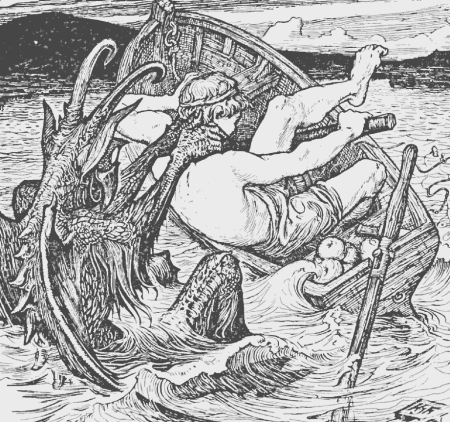
\includegraphics[scale=.4]{monsters/Water_1}
\end{center}

\MONSTER[
  NM=Toad Man,
  LK=monster-toad-man,
  SPD=Base,
  AT=weapon OR d4 / 1 Close,
  WK=d20,
  HD=3,
  PR=Average,
  SK=0,
  MR=Orderly,
  SV=9,
  SPL=0,
  TRT=\mylink{Zoological}{monster-trait-zoological}; \mylink{Slippery}{monster-trait-slippery}; \mylink{Amphibious}{monster-trait-amphibious}; \mylink{Canny}{monster-trait-canny}; \mylink{Leaping}{monster-trait-leaping},
  ACT=\mylink{Charge}{monster-action-charge}
  ]
Hilarious looking half-man, half-toad bipeds. Almost impossible to take seriously, except for the fact that they are armed and have no sense of humor. They prefer spears to make the best use of their leaping attacks.


\MONSTER[
  NM=Troglodyte,
  LK=monster-troglodyte,
  SPD=Base,
  AT=weapon OR d6 / 1 Close,
  WK=d24,
  HD=1,
  PR=Average,
  SK=0,
  MR=Orderly,
  SV=11,
  SPL=0,
  TRT=\mylink{Zoological}{monster-trait-zoological}; \mylink{Slippery}{monster-trait-slippery}; \mylink{Amphibious}{monster-trait-amphibious}; \mylink{Nocturnal}{monster-trait-nocturnal},
  ACT=None
 ]
Bipedal dwellers of caves and caverns, thought to be rejects from the \mylink{Veins of the Earth}{atlas-veins-earth}, a confusing mix of salamander and toad.  Trogs can spend an Action emitting a foul smelling gas that causes \mylink{Disgust}{effect-disgusted} to Adventurers who are Close unless they \SAVE{Toxins}.  The smell lasts for Minutes.



\newpage
\mysubsection{Arthropods}{monster-order-arthropods-detail}




\MONSTER[
  NM=Giant Ant,
  LK=monster-giant-ant,
  SPD=Base,
  AT=d10 1 Close,
  WK=d20,
  HD=3,
  PR=Average,
  SK=d4,
  MR=Orderly,
  SV=9,
  SPL=0,
  TRT=\mylink{Zoological}{monster-trait-zoological}; \mylink{Pack}{monster-trait-pack},
  ACT=None
 ]
\callout{
    Giants Ants have Fanatical morale when defending their homes.
}

\ed{Have you seen the movie "Them!" (1954) by any chance?  It's got Edmund Gwenn, the guy who plays Santa Claus in Capra's "Miracle on 34th Street".   You should check it out.}

Even normal ants have all kinds of ways of ruining your life.  If you feel your Adventurers are under-challenged, roll a d6 - the Giant Ant has:

\mynumlist {
    \item the \mylink{Venomous}{monster-trait-venomous} Trait.
    \item the \mylink{Acidic}{monster-trait-acidic} Trait.
    \item the \mylink{Flying}{monster-trait-flying} Trait.
    \item a paralytic bite. \SAVE{Toxins} if the Monster hits Flesh or be \mylink{Paralyzed}{effect-paralyzed} for \DUR{d4}.
    \item a stinger, can attack d10 2 Close (Either).
    \item the \mylink{Frenzied}{monster-trait-frenzied} Trait.
} 


\MONSTER[
  NM=Giant Beetle,
  LK=monster-giant-beetle,
  SPD=Slow,
  AT=d6+d8 1 Close,
  WK=d20,
  HD=5,
  PR=Strong,
  SK=d6,
  MR=Orderly,
  SV=7,
  SPL=0,
  TRT=\mylink{Zoological}{monster-trait-zoological},
  ACT=None
 ]
Boring beetles.  Deathwatch beetles.  Carrion beetles.  Long-horned beetles.  Predacious diving beetles.  Pleasing fungus beetles!  SOLDIER BEETLES!  No shit, there are even spider beetles (\myital{Anobiidae}). Long and short, use these stats as a base, but hit wikipedia.



\MONSTER[
  NM=Giant Centipede,
  LK=monster-giant-centipede,
  SPD=Fast,
  AT=d6 1 Close AND 1 dmg d6 Close (Either),
  WK=d16,
  HD=4,
  PR=Average,
  SK=0,
  MR=Orderly,
  SV=8,
  SPL=0,
  TRT=\mylink{Zoological}{monster-trait-zoological}; \mylink{Venomous}{monster-trait-venomous}; \mylink{Twitchy}{monster-trait-twitchy},
  ACT=None
 ]

\callout{
    Giant Centipede roll a d12 for \DEX tries.
}
Really fast giant crawling insects with far too many legs.   Makes a hissing sound as it flies down a tunnel to consume an Adventurer.

At the top of the Moment, roll a d6 - the Centipede can attack with this many legs in addition to gnawing with its horrific mouth parts. The legs only deal 1 point of damage, but they are also \mylink{Venomous}{monster-trait-venomous}.

\myimage{monsters/Arthropods}

\MONSTER[
  NM=Giant Spider,
  LK=monster-giant-spider,
  SPD=Fast,
  AT=d8 1 Nearby,
  WK=d20,
  HD=2,
  PR=Average,
  SK=0,
  MR=Orderly,
  SV=10,
  SPL=d4,
  TRT=\mylink{Zoological}{monster-trait-zoological}; \mylink{Venomous}{monster-trait-venomous},
  ACT=None
 ]
I mean ... it's a giant goddamn spider, anywhere between the size of a mastiff to the size of small van (increase \HD accordingly).  

Giant Spiders can use their Spell die to cast the \mylink{Secret: Web}{secrets-web} (only). 




\newpage

\mysubsection{Automatons}{monster-order-automatons-detail}


\MONSTER[
  NM=Iron Serpent,
  LK=monster-iron-serpent,
  SPD=Fast,
  AT=2d8 2 Close (Either),
  WK=d10,
  HD=7,
  PR=Average,
  SK=d8,
  MR=n/a,
  SV=5,
  SPL=0,
  TRT=\mylink{Mindless}{monster-trait-mindless}; \mylink{Unhallowed}{monster-trait-unhallowed}; \mylink{Twitchy}{monster-trait-twitchy},
  ACT=None
 ]

\callout{
    Iron Serpents roll a d12 for \DEX tries.
}

5 or 6 meter long serpents made of iron and Faith, usually set to guard tombs, shrines, or altars.  Extremely tough and greatly feared.  They are known to pursue intruders tirelessly until they are destroyed; unscrupulous Bands will send in linkboys, meat shields, and villagers to attract their attention ...

If an Iron Serpent strikes Flesh, the victim must \SAVE{Hexes};  Failure means a roll on the \mylink{Lesser Curses}{table-lesser-curses} table.




\MONSTER[
  NM=Living Statue,
  LK=monster-living-statue,
  SPD=Slow,
  AT=2d6 2 Close (Combined),
  WK=d12,
  HD=5,
  PR=Strong,
  SK=d8,
  MR=n/a,
  SV=7,
  SPL=0,
  TRT=\mylink{Mindless}{monster-trait-mindless}; \mylink{Unhallowed}{monster-trait-unhallowed}; \mylink{Strong}{monster-trait-strong},
  ACT=\mylink{Throw}{monster-action-throw}
  ]

\callout{
    Living Statues roll a d12 for \VIG tries.
}

Caryatids, maquettes, falla, and effigies; not quite \mylink{Golems}{miracle-golem}, but almost as powerful.  Often set to guard entrances, and mixed in with other (normal) statues of the same type.  Philosophers often place a \mylink{Talking Sigil}{inscription-sigil-talking}  on them, usually to shout out that there are intruders wandering about.

Living Statues can \mylink{Throw}{monster-action-throw} an Adventurer 20m.

\cbreak

\vspace*{5mm}

\MONSTER[
  NM=Robot,
  LK=monster-robot,
  SPD=Base,
  AT=d8 1 Nearby,
  WK=d20,
  HD=3,
  PR=Average,
  SK=d8,
  MR=n/a,
  SV=9,
  SPL=0,
  TRT=\mylink{Mindless}{monster-trait-mindless}; \mylink{Unhallowed}{monster-trait-unhallowed}; \mylink{Supportive}{monster-trait-supportive}; \mylink{Militant}{monster-trait-militant},
  ACT=None
 ]
Metal creatures of unknown provenance, of various heights and sizes.  They always appear in geometric binary sequences (2,4,8,16,etc).



\myimage{monsters/MonsterAutomaton}

\newpage
\mysubsection{Demons}{monster-order-demons-detail}

\MONSTER[
  NM=Ba'al,
  LK=monster-baal,
  SPD=Base,
  AT=d6+d8 1 Close,
  WK=d16,
  HD=5,
  PR=Average,
  SK=0,
  MR=Orderly,
  SV=7,
  SPL=0,
  TRT=\mylink{Unhallowed}{monster-trait-unhallowed}; \mylink{Terrifying}{monster-trait-terrifying}; \mylink{Chaotic}{monster-trait-chaotic}; \mylink{Nocturnal}{monster-trait-nocturnal}; \mylink{Otherworldly}{monster-trait-otherworldly}; \mylink{Strong}{monster-trait-strong}; \mylink{Slippery}{monster-trait-slippery}; \mylink{Leaping}{monster-trait-leaping},
  ACT=\mylink{Charge}{monster-action-charge}; \mylink{Rage}{monster-action-rage}
  ]
\callout{
    Ba'al roll a d12 for \VIG tries.
}

Powerful toad-demons who appear to have some sort of military structure that only they truly understand.  They have command over creatures of the \mylink{Amphibian}{monster-order-amphibians} Order, who use them as pawns or mounts.



\MONSTER[
  NM=Dretch,
  LK=monster-dretch,
  SPD=Base,
  AT=d6 1 Close,
  WK=d24,
  HD=1,
  PR=Weak,
  SK=0,
  MR=Cowardly,
  SV=11,
  SPL=0,
  TRT=\mylink{Unhallowed}{monster-trait-unhallowed}; \mylink{Terrifying}{monster-trait-terrifying}; \mylink{Chaotic}{monster-trait-chaotic}; \mylink{Nocturnal}{monster-trait-nocturnal}; \mylink{Otherworldly}{monster-trait-otherworldly}; \mylink{Pack}{monster-trait-pack}; \mylink{Stupid}{monster-trait-stupid},
  ACT=None
 ]
The lowest of demonkind, fodder for their constant battles.  Created from the cast off souls of Mortals in mockery of \TheAuthority.  Extremely stupid and possessing extraordinarily low self esteem.


\cbreak

\vspace*{5mm}

\MONSTER[
  NM=Naga,
  LK=monster-naga,
  SPD=Fast,
  AT=see below,
  WK=d10,
  HD=7,
  PR=Average,
  SK=d8,
  MR=Fanatical,
  SV=5,
  SPL=0,
  TRT=\mylink{Unhallowed}{monster-trait-unhallowed}; \mylink{Terrifying}{monster-trait-terrifying}; \mylink{Chaotic}{monster-trait-chaotic}; \mylink{Nocturnal}{monster-trait-nocturnal}; \mylink{Otherworldly}{monster-trait-otherworldly},
  ACT=None
 ]
\callout{
    Naga roll a d12 for \DEX tries.
}
Multi-armed half-snake, half Mortal demons, second only to Pit Fiends in power.  Fast, clever, and depraved.  They wield blades made of shadow in each of their hands, which blink in and out of existence.


At the top of each Moment, roll a d8.  The Naga is able to attack up to \SUM Close Adventurers (Either); each blade deals \SUM damage.  Note that the Naga can concentrate all of its attacks on a single hapless Adventurer if it so chooses.

\myimage{monsters/MonsterNaga}

\newpage

\end{multicols*}
\myimage{monsters/Demon2}
\begin{multicols*}{2}


\MONSTER[
  NM=Pit Fiend,
  LK=monster-pit-fiend,
  SPD=Base,
  AT=d24+d4 / 1d8 1 Close +1 Nearby,
  WK=d4,
  HD=9,
  PR=Strong,
  SK=d10,
  MR=n/a,
  SV=3,
  SPL=0,
  TRT=\mylink{Unhallowed}{monster-trait-unhallowed}; \mylink{Terrifying}{monster-trait-terrifying}; \mylink{Chaotic}{monster-trait-chaotic}; \mylink{Nocturnal}{monster-trait-nocturnal}; \mylink{Otherworldly}{monster-trait-otherworldly},
  ACT=\mylink{Rage}{monster-action-rage}; \mylink{Trample}{monster-action-trample}
  ]

I hope you saw The Fellowship of the Ring in the theaters, but maybe you were too young.  First time I saw the Balrog pop out to give Gandalf a run for his money, I actually spilled my popcorn.  The Pit Fiend is similar - just a giant, depraved, utterly evil, terrifying winged monster from the 9th plane of Hell.

The Pit Fiend strikes Close Adventurers with an abyssal blade (d24+4) that also deals \mylink{Rending}{weapon-attribute-rending} damage.  If an Adventurer is struck with the demon's whip (d8 Close or Nearby), they must \RBTRY{\DEX}{\VIG} or be immediately dragged to Close range.  The Pit Fiend can combine these into one Combat Maneuver if it wants i.e. hit an Adventurer with its whip and then strike with it sword.

Finally, Adventurers (and other Monsters) Close to the Pit Fiend must contend with its abyssal flames.  These flames deal d6 damage at the bottom of every Moment unless a \SAVE{Doom} try is made.








\MONSTER[
  NM=Vrock,
  LK=monster-vrock,
  SPD=Base,
  AT=2d6 2 Close (Combined),
  WK=d20,
  HD=3,
  PR=Average,
  SK=0,
  MR=Cowardly,
  SV=9,
  SPL=0,
  TRT=\mylink{Unhallowed}{monster-trait-unhallowed}; \mylink{Terrifying}{monster-trait-terrifying}; \mylink{Chaotic}{monster-trait-chaotic}; \mylink{Nocturnal}{monster-trait-nocturnal}; \mylink{Otherworldly}{monster-trait-otherworldly}; \mylink{Canny}{monster-trait-canny}; \mylink{Bloodthirsty}{monster-trait-bloodthirsty}; \mylink{Flying}{monster-trait-flying},
  ACT=None
 ]
A winged biped with the head of a toothed vulture and the talons of a raptor; extremely opportunistic, cowardly, and unpleasant.  While they have the \mylink{Flying}{monster-trait-flying} trait, they are really bad at it and require 2 Actions to move 1 range step.

\newpage


\mysubsection{Dinosaurs}{monster-order-dinosaurs-detail}


\MONSTER[
  NM=Allosaurus,
  LK=monster-allosaurus,
  SPD=Fast,
  AT=2d8 1 Close,
  WK=d12,
  HD=6,
  PR=Average,
  SK=d6,
  MR=Cowardly,
  SV=6,
  SPL=0,
  TRT=\mylink{Terrifying}{monster-trait-terrifying}; \mylink{Zoological}{monster-trait-zoological}; \mylink{Frenzied}{monster-trait-frenzied}; \mylink{Twitchy}{monster-trait-twitchy},
  ACT=None
 ]

\callout{
    Allosaurus roll a d12 for \DEX tries.
}
7.5 to 10.5 meter long, 1800kg bipedal theropod.  Like a T-Rex but juuuust a little smaller.




\MONSTER[
  NM=Plesiosarus,
  LK=monster-plesiosarus,
  SPD=Base,
  AT=d20 1 Close,
  WK=d10,
  HD=7,
  PR=Average,
  SK=d6,
  MR=Cowardly,
  SV=5,
  SPL=0,
  TRT=\mylink{Terrifying}{monster-trait-terrifying}; \mylink{Zoological}{monster-trait-zoological}; \mylink{Frenzied}{monster-trait-frenzied},
  ACT=None
 ]
5m long, 450kg marine dinosaur. They prefer warm waters, and can swim two ranges in a single Action.

\myimage{monsters/MonsterTrex}

\cbreak

\MONSTER[
  NM=Pteranodon,
  LK=monster-pteranodon,
  SPD=Base,
  AT=2d6 1 Close,
  WK=d16,
  HD=5,
  PR=Average,
  SK=0,
  MR=Cowardly,
  SV=7,
  SPL=0,
  TRT=\mylink{Terrifying}{monster-trait-terrifying}; \mylink{Zoological}{monster-trait-zoological}; \mylink{Frenzied}{monster-trait-frenzied}; \mylink{Flying}{monster-trait-flying},
  ACT=None
 ]
Clumsy flying dinosaurs with a 6-7 meter wingspan, can easily pick up something 100kg or less in its talons to drop it from a height, or attack with its snapping maw.


\MONSTER[
  NM=Triceratops,
  LK=monster-triceratops,
  SPD=Base,
  AT=2d8 1 Close,
  WK=d12,
  HD=6,
  PR=Strong,
  SK=d10,
  MR=Cowardly,
  SV=6,
  SPL=0,
  TRT=\mylink{Terrifying}{monster-trait-terrifying}; \mylink{Zoological}{monster-trait-zoological}; \mylink{Frenzied}{monster-trait-frenzied},
  ACT=\mylink{Trample}{monster-action-trample}
  ]
Quadrupedal dinosaur about 9m long and weighing a ridiculous 12 metric tons.  Generally pretty peaceful but short tempered if you decide to fuck with it (think rhinoceros but ... you know, a lot bigger).

Gores with its horns for 2d8 damage, but prefers to charge if it can.  If the Triceratops is able to move from Nearby to Close without taking damage, it will deal \MAX damage (16 points), and the unlucky Adventurer is knocked \mylink{Prone}{effect-prone} unless they can \RBTRY{\VIG}{\VIG}.


\MONSTER[
  NM=Tyrannosaurus Rex,
  LK=monster-tyrannosaurus-rex,
  SPD=Base,
  AT=d24+4 1 Close,
  WK=d8,
  HD=8,
  PR=Strong,
  SK=d10,
  MR=n/a,
  SV=4,
  SPL=0,
  TRT=\mylink{Terrifying}{monster-trait-terrifying}; \mylink{Zoological}{monster-trait-zoological}; \mylink{Frenzied}{monster-trait-frenzied},
  ACT=\mylink{Rage}{monster-action-rage}
  ]
The goddamn king.  If the T-Rex ever rolls \MAX damage, the Adventurer must make a \SAVE{Doom} or be immediately bitten in half.  This kills the Adventurer.

\newpage


\mysubsection{Dire Beasts}{monster-order-dire-beasts-detail}






\MONSTER[
  NM=Cannibal Ape,
  LK=monster-cannibal-ape,
  SPD=Base,
  AT=2d6 1 Close,
  WK=d16,
  HD=4,
  PR=Strong,
  SK=0,
  MR=Orderly,
  SV=8,
  SPL=0,
  TRT=\mylink{Berserk}{monster-trait-berserk}; \mylink{Zoological}{monster-trait-zoological}; \mylink{Cannibal}{monster-trait-cannibal},
  ACT=\mylink{Rage}{monster-action-rage}
  ]


\callout{
    Cannibal Apes roll a d12 for \VIG tries.
}
Favorite monster of Conan and other barbarian lit, fond of ripping creatures limb from limb and feasting on them while they're still alive and fresh.




\MONSTER[
  NM=Cave Bear,
  LK=monster-cave-bear,
  SPD=Slow,
  AT=2d6 1 Close AND d10 dmg 2 Close (Either),
  WK=d16,
  HD=5,
  PR=Strong,
  SK=d4,
  MR=Fanatical,
  SV=7,
  SPL=0,
  TRT=\mylink{Berserk}{monster-trait-berserk}; \mylink{Zoological}{monster-trait-zoological}; \mylink{Strong}{monster-trait-strong},
  ACT=\mylink{Charge}{monster-action-charge}
  ]
\callout{
    Cave Bears roll a d12 for \VIG tries.
}
3.5 meter long and 1,000kg of pure killing machine.  The Cave Bear can concentrate all 3 attacks on a single hapless Adventurer, or its bite (2d6) on one and claws (d10 / d10) on another.

\myimage{monsters/MonsterSabertooth}


\cbreak

\myimage{monsters/MonsterCaveBear}

\MONSTER[
  NM=Dire Wolf,
  LK=monster-dire-wolf,
  SPD=Fast,
  AT=d8 1 Close,
  WK=d20,
  HD=3,
  PR=Average,
  SK=0,
  MR=Orderly,
  SV=9,
  SPL=0,
  TRT=\mylink{Berserk}{monster-trait-berserk}; \mylink{Zoological}{monster-trait-zoological}; \mylink{Pack}{monster-trait-pack},
  ACT=None
 ]
2m long and 50kg, these killers like to hunt in packs.  Smarter than you think, they'll work together in ways Adventurers might not anticipate.

\MONSTER[
  NM=Sabertooth Cat,
  LK=monster-sabertooth-cat,
  SPD=Base,
  AT=d6+d8 1 Close AND 2d6 dmg 2 Close (Either),
  WK=d12,
  HD=6,
  PR=Average,
  SK=0,
  MR=Fanatical,
  SV=6,
  SPL=0,
  TRT=\mylink{Berserk}{monster-trait-berserk}; \mylink{Zoological}{monster-trait-zoological}; \mylink{Frenzied}{monster-trait-frenzied}; \mylink{Bloodthirsty}{monster-trait-bloodthirsty},
  ACT=None
 ]
King of the Dire Beasts, weighing in at 450kg and standing 1.2m at the shoulder.  The Sabertooth Cat can concentrate all 3 attacks on a single hapless Adventurer, or its bite (d6+d8) on one and claws (2d6) on another.  If both claws hit, the attack also \mylink{Rends}{weapon-attribute-rending}.



\newpage
\mysubsection{Giantkin}{monster-order-giantkin-detail}




\MONSTER[
  NM=Giant,
  LK=monster-giant,
  SPD=Slow,
  AT=d20 All Close (Distinct) OR see below,
  WK=d8,
  HD=8,
  PR=Strong,
  SK=0,
  MR=Cowardly,
  SV=4,
  SPL=0,
  TRT=\mylink{Strong}{monster-trait-strong}; \mylink{Stupid}{monster-trait-stupid},
  ACT=\mylink{Throw}{monster-action-throw}
  ]

\callout{
    Giants roll a d16 for \VIG tries.
}

Massive (4-6m tall) bipedal humanoids.  Giants prefer to fight with giant tree-trunks, massive broken stalagmites, dragon-bones etc. with giant (haha!) sweeping attacks, as well as kicking and stomping with their feet.  If an Adventurer is struck by one of these attacks, they must \RSTRY{\VIG} or be \mylink{Stunned}{effect-stunned} for \DUR{d4}.



In lieu of this sweeping attack, Giants can use one of the following Combat Maneuvers:


\mybullet {
    \item Grab up to d3 Close (Distinct) Adventurers with the \mylink{Throw}{monster-action-throw} Action to a distance of 30m.
    \item  Grab a large rock, wagon, cow, etc. and toss it somewhere Nearby.  All Adventurers Close to the point of impact must \RS : \VIG or \DEX (Adventurer's Choice) or be \mylink{Stunned}{effect-stunned} for \DUR{d4}.
    \item  Let out a massive roar.  All Adventurers Close to the sound must \SAVE{Doom} or be \mylink{Deafened}{effect-deafened} for \DUR{d4} and must immediately make an \INSANITY try.
    \item  Leap in the air and land with a crash.  All Adventurers Close must \RS : \VIG or \DEX (Adventurer's choice) or be knocked \mylink{Prone}{effect-prone}.
}

\cbreak

\vspace*{20mm}
\myimage{monsters/Giant}

\end{multicols*}
\begin{center}
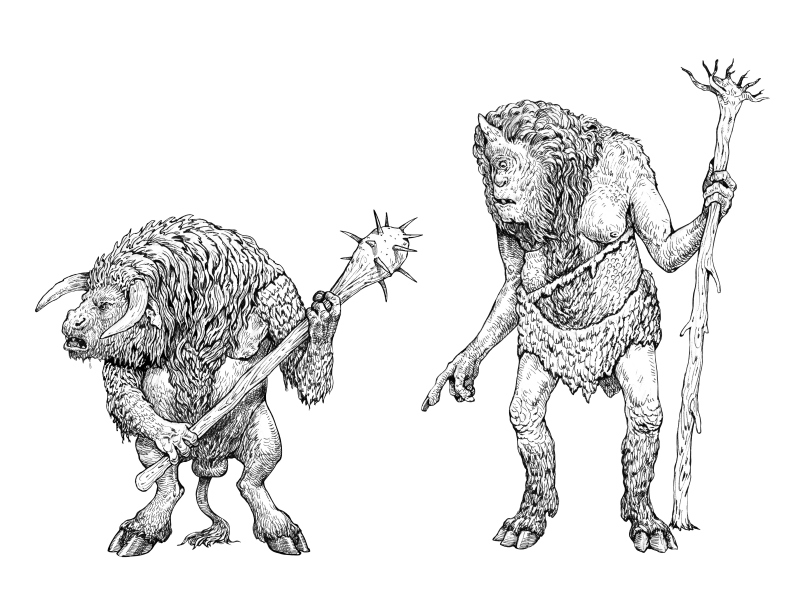
\includegraphics[width=.9\linewidth,keepaspectratio=true]{monsters/MonsterMinotaurOgre}
\end{center}

\begin{multicols*}{2}




\MONSTER[
  NM=Minotaur,
  LK=monster-minotaur,
  SPD=Base,
  AT=2d8 1 Close AND d10 2 Close (Combined),
  WK=d10,
  HD=7,
  PR=Strong,
  SK=0,
  MR=Fanatical,
  SV=5,
  SPL=0,
  TRT=\mylink{Strong}{monster-trait-strong}; \mylink{Stupid}{monster-trait-stupid}; \mylink{Berserk}{monster-trait-berserk},
  ACT=\mylink{Charge}{monster-action-charge}; \mylink{Rage}{monster-action-rage}
  ]
\callout{
    Minotaur roll a d12 for \VIG tries.
}
The bovine-headed abominations of myth, usually armed with a giant axe and a bad attitude.   The Minotaur can concentrate all 3 attacks on a single hapless Adventurer, or its axe (2d8) on one and horns (d10 / d10) on another.

\myimage{monsters/Minotaur}




\MONSTER[
  NM=Ogre,
  LK=monster-ogre,
  SPD=Slow,
  AT=2d6 1 Close,
  WK=d16,
  HD=4,
  PR=Strong,
  SK=0,
  MR=Fanatical,
  SV=8,
  SPL=0,
  TRT=\mylink{Strong}{monster-trait-strong}; \mylink{Stupid}{monster-trait-stupid}; \mylink{Bloodthirsty}{monster-trait-bloodthirsty},
  ACT=\mylink{Throw}{monster-action-throw}
  ]
\callout{
    Ogres roll a d12 for \VIG tries.
}


Smaller cousin of "true" giants, standing roughly 3m tall.  Somehow a whole lot stupider.  In emulation of their big brothers and sisters, they prefer clubs made out of massive tree branch which they use to pulverize their prey (Ogres surprisingly have very weak teeth and can only eat things that are in "paste" form).  1-in-6 ogres have 2 heads, another 1-in-6 have one eye.

Ogres can \mylink{Throw}{monster-action-throw} an Adventurer 10m.


\MONSTER[
  NM=Troll,
  LK=monster-troll,
  SPD=Base,
  AT=2d6 1 Close,
  WK=d12,
  HD=6,
  PR=Strong,
  SK=0,
  MR=Orderly,
  SV=6,
  SPL=0,
  TRT=\mylink{Strong}{monster-trait-strong}; \mylink{Stupid}{monster-trait-stupid}; \mylink{Nocturnal}{monster-trait-nocturnal},
  ACT=None
 ]
\callout{
Trolls are Cowardly when facing fire.

Trolls heal 3 Health at the bottom of every Moment.
}

\myimage{monsters/Troll}

Green, gray, or blue skinned Monsters that inhabit caves, swamps, and dark forests.  Nasty bits of work, but deeply afraid of fire.

Trolls will heal 3 Health at the bottom of every Moment if the damage source was not fire.  



\MONSTER[
  NM=Wendigo,
  LK=monster-wendigo,
  SPD=Base,
  AT=2d6 1 Close,
  WK=d16,
  HD=5,
  PR=Average,
  SK=0,
  MR=Fanatical,
  SV=7,
  SPL=0,
  TRT=\mylink{Strong}{monster-trait-strong}; \mylink{Stupid}{monster-trait-stupid}; \mylink{Terrifying}{monster-trait-terrifying}; \mylink{Cannibal}{monster-trait-cannibal},
  ACT=\mylink{Rage}{monster-action-rage}
  ]
\callout{
    Wendigo roll a d12 for \VIG tries.
}

Malevolent, cannibalistic, and supernatural Monsters usually found in cold regions, or regions where famine is rampant. Descriptions by the famished and insane survivors of Wendigo attacks differ, but generally agree on the form of a tall (2.5m), gaunt beast with long claws, black eyes, and a mouth with too many teeth.


\newpage

\mysubsection{Goblinoids}{monster-order-goblinoids-detail}

\MONSTER[
  NM=Bugbear,
  LK=monster-bugbear,
  SPD=Base,
  AT=d10 1 Close,
  WK=d20,
  HD=3,
  PR=Strong,
  SK=0,
  MR=Fanatical,
  SV=9,
  SPL=0,
  TRT=\mylink{Nocturnal}{monster-trait-nocturnal}; \mylink{Canny}{monster-trait-canny}; \mylink{Bloodthirsty}{monster-trait-bloodthirsty},
  ACT=\mylink{Rage}{monster-action-rage}
  ]
Giant hairy goblins that attack with iron-hard claws.  If a Bugbear successfully hits an Adventurer, they can \mylink{Rend}{weapon-attribute-rending} instead of dealing damage.  They like to target heavily armored Adventurers and peel them like grapes.




\MONSTER[
  NM=Gnoll,
  LK=monster-gnoll,
  SPD=Fast,
  AT=weapon or d6 / 1 Close,
  WK=d20,
  HD=2,
  PR=Average,
  SK=0,
  MR=Orderly,
  SV=10,
  SPL=0,
  TRT=\mylink{Nocturnal}{monster-trait-nocturnal}; \mylink{Canny}{monster-trait-canny}; \mylink{Pack}{monster-trait-pack}; \mylink{Militant}{monster-trait-militant},
  ACT=\mylink{Charge}{monster-action-charge}
  ]
Militant hyena-headed goblinoids that prefer hit-and-run tactics.  They prefer spears and flails for their dirty work.



\MONSTER[
  NM=Goblin,
  LK=monster-goblin,
  SPD=Fast,
  AT=weapon or d4 / 1 Close,
  WK=d24,
  HD=1,
  PR=Weak,
  SK=0,
  MR=Cowardly,
  SV=11,
  SPL=0,
  TRT=\mylink{Nocturnal}{monster-trait-nocturnal}; \mylink{Canny}{monster-trait-canny}; \mylink{Pack}{monster-trait-pack},
  ACT=\mylink{Charge}{monster-action-charge}; \mylink{Rout}{monster-action-rout}
  ]
Tiny evil chattering critters that work well together (up to a point) to take down Adventurers.



\MONSTER[
  NM=Hobgoblin,
  LK=monster-hobgoblin,
  SPD=Base,
  AT=weapon 1 Close OR weapon 1 Far-Away (Bow) OR d4 1 Close,
  WK=d24,
  HD=2,
  PR=Average,
  SK=0,
  MR=Orderly,
  SV=10,
  SPL=0,
  TRT=\mylink{Nocturnal}{monster-trait-nocturnal}; \mylink{Canny}{monster-trait-canny}; \mylink{Militant}{monster-trait-militant},
  ACT=\mylink{Charge}{monster-action-charge}
  ]
Bigger and more militant than the Goblins they lead.   "Hobs" are usually armed with short bows in addition to melee weapons, and if unarmed are still able to strike with their hands and feet for 3 damage.




\MONSTER[
  NM=Kobold,
  LK=monster-kobold,
  SPD=Base,
  AT=d4 1 Close OR d4 1 Nearby,
  WK=d24,
  HD=0,
  PR=Weak,
  SK=0,
  MR=Cowardly,
  SV=12,
  SPL=0,
  TRT=\mylink{Nocturnal}{monster-trait-nocturnal}; \mylink{Canny}{monster-trait-canny},
  ACT=\mylink{Rout}{monster-action-rout}
  ]
Dog-headed tiny critters, about the size of a Pooka.  Kobolds fight with improvised weapons with surprising skill - broken bottles, sacks of rusty nails, rolling pins, sharp sticks, etc  They can throw these weapons in addition to using them in close combat.  Regardless of the weapon, it deals d4 damage.

\myimage{monsters/Kobold}

If they are disarmed or lose their weapon, they may spend an Action to improvise a new one.  





\MONSTER[
  NM=Orc,
  LK=monster-orc,
  SPD=Base,
  AT=d6 1 Close,
  WK=d24,
  HD=1,
  PR=Strong,
  SK=0,
  MR=Fanatical,
  SV=11,
  SPL=0,
  TRT=\mylink{Nocturnal}{monster-trait-nocturnal}; \mylink{Canny}{monster-trait-canny}; \mylink{Cannibal}{monster-trait-cannibal}; \mylink{Militant}{monster-trait-militant},
  ACT=\mylink{Charge}{monster-action-charge}
  ]
Pig-faced classics.  Very reliable (to the Arbiter, I mean).  Often stuck guarding chests in 10'x10' rooms.  Always deal d6 damage whether they're armed or not. 

\newpage
\mysubsection{Goos}{monster-order-goos-detail}




\MONSTER[
  NM=Black Jelly,
  LK=monster-black-jelly,
  SPD=Slow,
  AT=d10 1 Close,
  WK=d20,
  HD=3,
  PR=Average,
  SK=0,
  MR=n/a,
  SV=9,
  SPL=0,
  TRT=\mylink{Mindless}{monster-trait-mindless}; \mylink{Amorphous}{monster-trait-amorphous}; \mylink{Splitting}{monster-trait-splitting}; \mylink{Acidic}{monster-trait-acidic},
  ACT=None
 ]
\callout{
    At the start of every Moment, roll a d3.  The result is the Gelatinous Cube's Soak for that Moment: 1 (d4), 2 (d6). 
}
Big, oily, black, acidic sentient goo.   Cold-based damage dealt to a Black Jelly will not cause it to Split.

\myimage{monsters/Goo_3}


\MONSTER[
  NM=Gelatinous Cube,
  LK=monster-gelatinous-cube,
  SPD=Slow,
  AT=see below,
  WK=d16,
  HD=4,
  PR=Average,
  SK=see below,
  MR=n/a,
  SV=8,
  SPL=0,
  TRT=\mylink{Mindless}{monster-trait-mindless}; \mylink{Amorphous}{monster-trait-amorphous}; \mylink{Splitting}{monster-trait-splitting},
  ACT=None
 ]
\callout{
    At the start of every Moment, roll a d3.  The result is the Gelatinous Cube's Soak for that Moment: 1 (d4), 2 (d6), 3 (d8). 
}
Opaque cube-shaped wandering goos.  

Creatures hit by a Gelatinous Cube are engulfed unless they win a \RB : \VIG or \DEX try (Adventurer choice) vs. the Gelatinous Cube's \VIG.

Engulfed creatures take ongoing d6 damage at the top of every Moment.  It's possible to cut your way out, but Attack \RO tries are made at -4 while engulfed, and damage dealt is -2 (minimum 1).  Spellcasting is impossible while engulfed.

Successful attacks made from inside the Gelatinous Cube will not cause it to Split.


\MONSTER[
  NM=Green Slime,
  LK=monster-green-slime,
  SPD=Slow,
  AT=d8 1 Close,
  WK=d20,
  HD=2,
  PR=Average,
  SK=d4,
  MR=n/a,
  SV=10,
  SPL=0,
  TRT=\mylink{Mindless}{monster-trait-mindless}; \mylink{Amorphous}{monster-trait-amorphous}; \mylink{Splitting}{monster-trait-splitting},
  ACT=None
 ]
Green, sticky, wet, sucking goos.


\MONSTER[
  NM=Ochre Mold,
  LK=monster-ochre-mold,
  SPD=Slow,
  AT=d12 1 Close,
  WK=d16,
  HD=5,
  PR=Average,
  SK=0,
  MR=n/a,
  SV=7,
  SPL=0,
  TRT=\mylink{Mindless}{monster-trait-mindless}; \mylink{Amorphous}{monster-trait-amorphous}; \mylink{Splitting}{monster-trait-splitting}; \mylink{Venomous}{monster-trait-venomous},
  ACT=None
 ]

\callout{
    At the start of every Moment, roll a d3.  The result is the Gelatinous Cube's Soak for that Moment: 1 (d4), 2 (d6), 3 (d8), 4 (d10). 
}

Toxic orange-yellow furry molds.  Fire-based damage dealt to an Ochre Mold will not cause it to Split.

\newpage
\mysubsection{Horrors}{monster-order-horrors-detail}




\MONSTER[
  NM=Ghast,
  LK=monster-ghast,
  SPD=Base,
  AT=d8 1 Close,
  WK=d16,
  HD=4,
  PR=Average,
  SK=0,
  MR=Orderly,
  SV=8,
  SPL=0,
  TRT=\small{\mylink{Unhallowed}{monster-trait-unhallowed}; \mylink{Terrifying}{monster-trait-terrifying}; \mylink{Nocturnal}{monster-trait-nocturnal}; \mylink{Bloodthirsty}{monster-trait-bloodthirsty}; \mylink{Leaping}{monster-trait-leaping}},
  ACT=None
 ]
\flavor{... the ghasts, those repulsive beings which die in the light, and which live in the vaults of Zin and leap on long hind legs like kangaroos ... After a moment something about the size of a small horse hopped out into the grey twilight, and Carter turned sick at the aspect of that scabrous and unwholesome beast, whose face is so curiously human despite the absence of a nose, a forehead, and other important particulars ... \Tilde H.P. Lovecraft }

Strikes from a Ghast are paralytic.  If a Ghast strikes Flesh, the Adventurer must \RS: \FOC\@ - failure means they are \mylink{Paralyzed}{effect-paralyzed} for \DUR{d4}.

\MONSTER[
  NM=Ghoul,
  LK=monster-ghoul,
  SPD=Fast,
  AT=d8 1 Close,
  WK=d20,
  HD=2,
  PR=Average,
  SK=0,
  MR=Cowardly,
  SV=10,
  SPL=0,
  TRT=\small{\mylink{Unhallowed}{monster-trait-unhallowed}; \mylink{Terrifying}{monster-trait-terrifying}; \mylink{Nocturnal}{monster-trait-nocturnal}; \mylink{Pack}{monster-trait-pack}; \mylink{Cannibal}{monster-trait-cannibal}},
  ACT=None
 ]
Cannibalistic bipedal horrors that possess large toothed mouths and barbed tongues. They are able to imitate voices and sounds they have heard (though they can only speak 1 word at most). They frequently use this ability to lure unwary Adventurers into their lairs.

Ghouls usually travel in packs of 2 to 7.

\cbreak

\myimage{monsters/Werewolf}

\MONSTER[
  NM=Werewolf,
  LK=monster-werewolf,
  SPD=Fast,
  AT=d6+d8 1 Close,
  WK=d16,
  HD=5,
  PR=Average,
  SK=0,
  MR=Fanatical,
  SV=7,
  SPL=0,
  TRT=\small{\mylink{Unhallowed}{monster-trait-unhallowed}; \mylink{Terrifying}{monster-trait-terrifying}; \mylink{Nocturnal}{monster-trait-nocturnal}; \mylink{Otherworldly}{monster-trait-otherworldly}},
  ACT=None
 ]

"Werewolf" covers pretty much any lycanthrope - half Mortal, half Monstrous creatures.  They appear to be some sort of living virus.

If a Werewolf's attack hits Flesh, roll the Adventurer's \SAVE{Doom} in secret.  Failure means the virus has spread to them, and will manifest itself in d6 Sessions (or whenever you think it's funniest).


\end{multicols*}
\newpage


\myimage{monsters/MonsterGhoul}

\flavor {
Cold be hand and heart and bone ~\\
and cold be sleep under stone ~\\
never more to wake on stony bed ~\\
never, till the Sun fails and the Moon is dead. ~\\

In the black wind the stars shall die ~\\
and still be gold here let them lie ~\\
till the Dark Lord lifts his hand ~\\
over dead sea and withered land.  ~\\
\Tilde J.R.R. Tolkien
}



\MONSTER[
  NM=Wight,
  LK=monster-wight,
  SPD=Base,
  AT=d10 1 Close,
  WK=d20,
  HD=3,
  PR=Average,
  SK=0,
  MR=Orderly,
  SV=9,
  SPL=0,
  TRT=\mylink{Unhallowed}{monster-trait-unhallowed}; \mylink{Terrifying}{monster-trait-terrifying}; \mylink{Nocturnal}{monster-trait-nocturnal}; \mylink{Frenzied}{monster-trait-frenzied},
  ACT=None
 ]

Shadowy, terrifying horrors that live in barrows, graveyards, and crypts.  If a Mortal dies from a Wight's attack, their soul does not travel to \mylink{Limbo}{the-afterlife}; it is hurled into the Void and destroyed. The physical body becomes a Wight that haunts the place of their death.

\newpage
\begin{multicols*}{2}
\mysubsection{Plantlife}{monster-order-plantlife-detail}




\MONSTER[
  NM=Fungoid,
  LK=monster-fungoid,
  SPD=Base,
  AT=weapon or d3 / 1 Close,
  WK=d24,
  HD=0,
  PR=Average,
  SK=0,
  MR=Orderly,
  SV=d4,
  SPL=0,
  TRT=\mylink{Mindless}{monster-trait-mindless}; \mylink{Supportive}{monster-trait-supportive}; \mylink{Pack}{monster-trait-pack}; \mylink{Cannibal}{monster-trait-cannibal},
  ACT=None
 ]
Tiny bipedal toadstools that work together in packs to take down their prey.  It's difficult to imagine a more humiliating death.




\MONSTER[
  NM=Orchidman,
  LK=monster-orchidman,
  SPD=Base,
  AT=see below / 1 Close,
  WK=d20,
  HD=3,
  PR=Average,
  SK=0,
  MR=Orderly,
  SV=9,
  SPL=0,
  TRT=\mylink{Mindless}{monster-trait-mindless},
  ACT=None
 ]

The Orchidmen are plant creatures that resemble men with the heads of carnivorous orchids. They move unsteadily, as if intoxicated, and secrete a corrosive acid infused with mind-altering pheromones from their pits. These pheromones incite a tangible sense of desire in Mortals and Unseelie alike.

Orchidmen only try to grapple Adventurers. If successful, the Adventurer must \RS : \FOC at the top of the Moment or willingly plunge their head into the Orchidman's pit, taking d8 damage immediately.  At the top of each Moment thereafter, they must \SAVE{Doom} or continue to bathe in the Orchidman's ... juices ... taking d8 damage at the bottom of the Moment.  If the Adventurer is wearing a helmet, they may "sunder" it to prevent one Moment's worth of damage.

\cbreak

When the Orchidman is slain it explodes, spraying everyone Close with a caustic goo that removes 1 \UD of Armor, or deals d4 damage unless a \SAVE{Doom} is made.

\myimage{monsters/Plants}





\MONSTER[
  NM=Swamp Thing,
  LK=monster-swamp-thing,
  SPD=Slow,
  AT=d10 3 Nearby (Either),
  WK=d16,
  HD=5,
  PR=Strong,
  SK=d6,
  MR=Orderly,
  SV=7,
  SPL=0,
  TRT=\mylink{Mindless}{monster-trait-mindless}; \mylink{Strong}{monster-trait-strong}; \mylink{Slippery}{monster-trait-slippery},
  ACT=\mylink{Grapple}{monster-action-grapple}
  ]

\callout{
    Swamp Things roll a d12 for \VIG tries.
}

A mass of putrefying peat, mud, roots, and branches in humanoid form.  They shoot tendrils from their fists and can simultaneously attack up to 3 Adventurers Close or Nearby.  On a 1-in-6, the tendrils have thorns - if they do, they cause \mylink{Bleeding}{effect-bleeding} if they strike Flesh.

\newpage
\mysubsection{Reptiles}{monster-order-reptiles-detail}




\MONSTER[
  NM=Giant Lizard,
  LK=monster-giant-lizard,
  SPD=Base,
  AT=d10 1 Close,
  WK=d20,
  HD=3,
  PR=Average,
  SK=d4,
  MR=Orderly,
  SV=9,
  SPL=0,
  TRT=\mylink{Zoological}{monster-trait-zoological}; \mylink{Frenzied}{monster-trait-frenzied},
  ACT=None
 ]
Giant iguanas, chameleons, geckos, skinks, monitor lizards, gila monsters, and burrowing worm lizards (holy shit, that's a thing).  Use these stats as a base, but let your imagination go wild.




\MONSTER[
  NM=Giant Snake,
  LK=monster-giant-snake,
  SPD=Fast,
  AT=d8 1 Close,
  WK=d16,
  HD=4,
  PR=Average,
  SK=d6,
  MR=Orderly,
  SV=8,
  SPL=0,
  TRT=\mylink{Zoological}{monster-trait-zoological}; \mylink{Frenzied}{monster-trait-frenzied}; \mylink{Venomous}{monster-trait-venomous},
  ACT=None
 ]
I mean ... I feel like there's not much to say about giant fuck-off snakes.  


\MONSTER[
  NM=Lizard Man,
  LK=monster-lizard-man,
  SPD=Base,
  AT=weapon or d6 / 1 Close,
  WK=d20,
  HD=2,
  PR=Average,
  SK=0,
  MR=Orderly,
  SV=10,
  SPL=0,
  TRT=\mylink{Zoological}{monster-trait-zoological}; \mylink{Frenzied}{monster-trait-frenzied}; \mylink{Militant}{monster-trait-militant},
  ACT=None
 ]


Lizard-like bipeds, militant and intelligent.  They'll often ride Giant Lizards into combat.

\cbreak

\vspace*{20mm}
\myimage{monsters/Reptiles}

\newpage
\mysubsection{Shades}{monster-order-shades-detail}

\myimage{monsters/Unquiet_Spirit}





\MONSTER[
  NM=Banshee,
  LK=monster-banshee,
  SPD=Base,
  AT=d4 1 Close,
  WK=d12,
  HD=6,
  PR=Average,
  SK=0,
  MR=Orderly,
  SV=6,
  SPL=0,
  TRT=\small{\mylink{Unhallowed}{monster-trait-unhallowed}; \mylink{Terrifying}{monster-trait-terrifying}; \mylink{Spectral}{monster-trait-spectral}; \mylink{Otherworldly}{monster-trait-otherworldly}},
  ACT=None
 ]
Long lanky hair covers a face you can never seem to make out, a rotting gray cloak over a bottle green dress.  Any Adventurer struck by a Banshee must make an \INSANITY try in addition to the damage taken.

If a Banshee is slain, it will let out an ear-splitting keening - all creatures (Adventurer or Monster alike) must immediately \SAVE{Doom} or fall to 0 Flesh (meaning they must roll their \DEATH at the top of the Moment).

\MONSTER[
  NM=Shadow,
  LK=monster-shadow,
  SPD=Base,
  AT=d10 1 Close,
  WK=d16,
  HD=4,
  PR=Average,
  SK=0,
  MR=Orderly,
  SV=8,
  SPL=0,
  TRT=\small{\mylink{Unhallowed}{monster-trait-unhallowed}; \mylink{Terrifying}{monster-trait-terrifying}; \mylink{Spectral}{monster-trait-spectral}; \mylink{Otherworldly}{monster-trait-otherworldly}; \mylink{Bloodthirsty}{monster-trait-bloodthirsty}},
  ACT=None
 ]
Enraged and malicious spirits that lurk in dark corners of crypts and tombs (treat as Invisible while they are hiding under these conditions). Shadows are attracted to injured or bleeding Adventurers, and will try to pick them off first.





\MONSTER[
  NM=Unquiet Spirit,
  LK=monster-unquiet-spirit,
  SPD=Base,
  AT=d4 + Life Drain / 1 Close,
  WK=varies,
  HD=0,
  PR=Weak,
  SK=0,
  MR=Orderly,
  SV=12,
  SPL=0,
  TRT=\mylink{Unhallowed}{monster-trait-unhallowed}; \mylink{Terrifying}{monster-trait-terrifying}; \mylink{Spectral}{monster-trait-spectral}; \mylink{Otherworldly}{monster-trait-otherworldly},
  ACT=None
 ]


Unquiet spirits sap energy from their victims unless the victim \RBTRY{\FOC}{\FOC}. If the Adventurer fails, roll a d6:


\mynumlist {
    \item Shift your \PRE \DCDOWN.
    \item Shift your \AWA \DCDOWN.
    \item Shift your \CLR \DCDOWN.
    \item Shift your \TAL \DCDOWN.
    \item d4 Damage to Grit.
    \item 1 Damage directly to Flesh (cannot be blocked by Armor).
}


\callout {
Apparition: 1HD, Save d4, Wk d24, Foc: d6
Spook: 3HD, Save d8+1, Wk d20, Foc: d8
Phantom: 5HD, Save d12+2, Wk d16, Foc: d10
Ghost: 7HD, Save d16+3, Wk d10, Foc: d12
}

\newpage

\end{multicols*}
\mysubsection{Swarms}{monster-order-swarms-detail}
\myimage{monsters/Locust}
\begin{multicols*}{2}




\MONSTER[
  NM=Insect Swarm,
  LK=monster-insect-swarm,
  SPD=Base,
  AT=\HD x2 All Close,
  WK=d20,
  HD=0,
  PR=Average,
  SK=0,
  MR=n/a,
  SV=d8+1,
  SPL=0,
  TRT=\mylink{Mindless}{monster-trait-mindless}; \mylink{Zoological}{monster-trait-zoological}; \mylink{Swarming}{monster-trait-swarming},
  ACT=None
 ]
Swarms of carnivorous beetles, biting ants, spiders, etc.

If an Insect Swarm strikes an Adventurer's Flesh, add an additional +2 damage.




\MONSTER[
  NM=Snake Swarm,
  LK=monster-snake-swarm,
  SPD=Base,
  AT=\HD x2 All Close,
  WK=d20,
  HD=0,
  PR=Average,
  SK=0,
  MR=n/a,
  SV=12,
  SPL=0,
  TRT=\mylink{Mindless}{monster-trait-mindless}; \mylink{Zoological}{monster-trait-zoological}; \mylink{Swarming}{monster-trait-swarming},
  ACT=None
 ]
Swarms of venomous snakes of all shapes and kinds.

If a Snake Swarm strikes an Adventurer's Flesh, they must roll a \SAVE{Toxins} or suffer the effects of a Noxious (d6) \mylink{Toxin}{malignants-toxins}.


\MONSTER[
  NM=Vermin Swarm,
  LK=monster-vermin-swarm,
  SPD=Base,
  AT=\HD x2 All Close,
  WK=d20,
  HD=0,
  PR=Average,
  SK=0,
  MR=n/a,
  SV=d8+1,
  SPL=0,
  TRT=\mylink{Mindless}{monster-trait-mindless}; \mylink{Zoological}{monster-trait-zoological}; \mylink{Swarming}{monster-trait-swarming},
  ACT=None
 ]
Swarms of rats, mice, and other carrion feeders. The Swarm will deal 2x\HD of damage to all creatures Close to it (so if you create a 2 \HD swarm, it will deal 4 damage).

If a Vermin Swarm strikes an Adventurer's Flesh, the Adventurer must \SAVE{Toxins} or roll on the \mylink{Diseases}{vulgate-medicine-diseases} table.

\newpage
\mysubsection{Walking Dead}{monster-order-walking-dead-detail}




\MONSTER[
  NM=Lich,
  LK=monster-lich,
  SPD=Base,
  AT=see below,
  WK=d4,
  HD=9,
  PR=Weak,
  SK=0,
  MR=n/a,
  SV=3,
  SPL=0,
  TRT=\mylink{Mindless}{monster-trait-mindless}; \mylink{Dead}{monster-trait-dead}; \mylink{Unhallowed}{monster-trait-unhallowed}; \mylink{Terrifying}{monster-trait-terrifying}; \mylink{Otherworldly}{monster-trait-otherworldly},
  ACT=None
 ]
A once-Mortal who has performed the profane right of \mylink{Lichdom}{occultism-lichdom}. You are encouraged to stat an appropriately leveled Adventurer, but if you're in a pinch, the following should work.

Each ability below has a \UD attached to it.  Using one of these abilities counts as a Combat action:

\mybullet {
    \item  Soulfire (d6): d24+4 damage to d4 Nearby creatures who fail a \\~ \SAVE{Hexes}.
    \item  Level Drain (d4): d4 Nearby creatures must \SAVE{Hexes} or drop all four facets of their \mylink{Personality}{adventurer-personality} \DCDOWN.
    \item  Mangle Flesh (d4): One Nearby creature must \SAVE{Hexes} or reduce their \VIG or \DEX  \DCDOWN (player's choice).
    \item  Ray of Death (d4): One Nearby creature must \SAVE{Hexes} or be reduced to 0 Flesh (and roll their \DEATH at the top of the Moment).
}


Additionally, a Lich is usually armed with a \mylink{Magic Staff}{wonder-staff-magic} or \mylink{Magic Sword}{wonder-sword-magic} of suitable power. 

If a Lich is slain but its phylactery remains intact, it will reform at the next sunset.  If it reforms, all of its \UD and Health reset to normal.

\cbreak

\vspace*{20mm}
\myimage{monsters/Lich}
\newpage

\MONSTER[
  NM=Skeleton,
  LK=monster-skeleton,
  SPD=Base,
  AT=weapon or d4 / 1 Close,
  WK=d24,
  HD=1,
  PR=Average,
  SK=d4,
  MR=n/a,
  SV=11,
  SPL=0,
  TRT=\mylink{Mindless}{monster-trait-mindless}; \mylink{Dead}{monster-trait-dead}; \mylink{Unhallowed}{monster-trait-unhallowed},
  ACT=None
 ]
The classic - skeletal remains of Mortals, bent to unholy purpose. Against Stabbing weapons, skeletons have d4 Soak (otherwise, damage is normal).

\myimage{monsters/Skeleton}





\MONSTER[
  NM=Vampire,
  LK=monster-vampire,
  SPD=Base,
  AT=2d6  1 Close,
  WK=d10,
  HD=7,
  PR=Average,
  SK=0,
  MR=n/a,
  SV=5,
  SPL=3d4,
  TRT=\mylink{Mindless}{monster-trait-mindless}; \mylink{Dead}{monster-trait-dead}; \mylink{Unhallowed}{monster-trait-unhallowed}; \mylink{Bloodthirsty}{monster-trait-bloodthirsty}; \mylink{Cannibal}{monster-trait-cannibal},
  ACT=None
 ]


Bloodthirsty fanged walking dead (everyone has an idea of what a vampire looks like, from Nosferatu to Dracula, so go with whatever makes sense for your game).

Once per Combat, in lieu of an attack, the vampire may attempt to charm a Nearby victim.  The victim must make a \SAVE{Hexes} - if they Fail, they immediately fall under the Vampire's sway for \DUR{d6}. A Vampiric Charm is particularly potent, and the victim will fight for the Vampire or willingly allow themselves to be bitten - though they will stop short of taking their own life.

If a Vampire's attack hits Flesh, the victim is affected by \mylink{Bleeding}{effect-bleeding}.  The Vampire heals 1 Health at the top of every Moment for every creature Close to it that is Bleeding.

If reduced to 0 Health - and not in a manner appropriate for truly killing vampires in your game - the vampire turns into a cloud of mist and escapes.


\MONSTER[
  NM=Zombie,
  LK=monster-zombie,
  SPD=Slow,
  AT=d8 1 Close,
  WK=d20,
  HD=2,
  PR=Strong,
  SK=0,
  MR=n/a,
  SV=10,
  SPL=0,
  TRT=\mylink{Mindless}{monster-trait-mindless}; \mylink{Dead}{monster-trait-dead}; \mylink{Unhallowed}{monster-trait-unhallowed}; \mylink{Pack}{monster-trait-pack}; \mylink{Cannibal}{monster-trait-cannibal},
  ACT=\mylink{Grapple}{monster-action-grapple}
  ]
Unless they get \mylink{the Drop}{combat-drop} on you, you always win Init against a Zombie. 

The initial attack from a Zombie should be treated as a \mylink{Grappling}{monster-action-grapple} attack.  If they succeed, their bite automatically hits during their turn in the following Moments.

\begin{center}
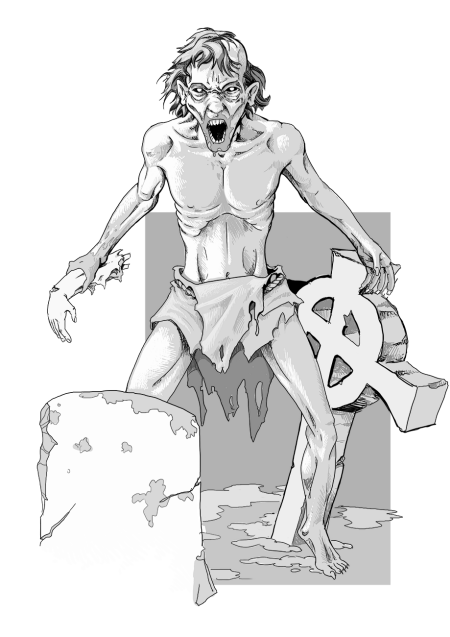
\includegraphics[scale=.3]{monsters/Zombie}
\end{center}
\newpage
% MONSTERS END



\mysubsection{Elementals}{monster-elementals}

\callout{
 Elemental Monsters immune to all Arcana except the \mylink{Secrets of Elements}{arcana-wizardry-secrets}.
}





\MONSTER[
  NM=Lesser Elemental,
  LK=monster-lesser-elemental,
  SPD=Base,
  AT=d6+d8 1 Close,
  WK=d16,
  HD=5,
  PR=Average,
  SK=d4,
  MR=n/a,
  SV=7,
  SPL=0,
  TRT=\mylink{Otherworldly}{monster-trait-otherworldly},
  ACT=None
]
Lesser elementals come in 6 types: Ice, Blood, Mud, Smoke, Dust, and Clay

\mybullet {
  \item \mybold{Ice} Wind and Water. Ice elementals freeze the ground Close to themselves - anyone who tries an Attack against the elemental while Close must \RSTRY{\DEX} after their attack (hit or miss) or fall Prone.

  \item \mybold{Blood} Water and Fire.  If a Blood elemental attack hits Flesh, it heals for a number of points equal to the amount of Flesh damaged.

  \item \mybold{Mud} Earth and Water.  The ground near the Mud elemental turns to knee deep muck.  Anyone Close to the elemental cannot move without a successful \RSTRY{\VIG}.

  \item \mybold{Smoke} Fire and Wind.  When a Smoke elemental is struck the first time in Combat, roll a d4 - this number of illusory Smoke elementals appear around it.  The illusions have only 1 Health, but any attack hits one of these illusions first (area of effect spells can potentially wipe them all out).

  \item \mybold{Dust} Wind and Earth.  Each time a Dust Elemental is struck by a Close physical attack, the attacker must roll a \SAVE{Doom} or be \mylink{Blinded}{effect-blinded} for \DUR{d4}.

  \item \mybold{Clay} Earth and Fire.  Whenever a Clay elemental is struck by a weapon, the attacker must \RSTRY{\VIG} or their weapon is stuck in the Clay elemental, and cannot be freed until the creature is slain.
}

\begin{center}
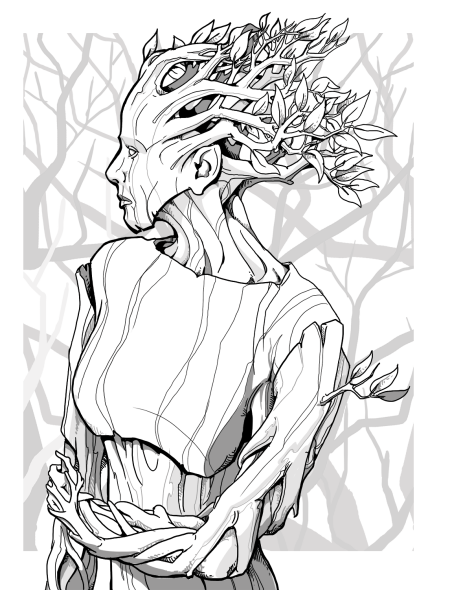
\includegraphics[scale=.3]{monsters/Elemental_1}
\end{center}

\MONSTER[
  NM=Greater Elemental,
  LK=monster-greater-elemental,
  SPD=Base,
  AT=d20 1 Close,
  WK=d10,
  HD=7,
  PR=Strong,
  SK=d8,
  MR=n/a,
  SV=5,
  SPL=0,
  TRT=\mylink{Otherworldly}{monster-trait-otherworldly},
  ACT=None
]
Greater elementals come in 4 types: Water, Wind, Fire, and Earth.  Each one has their own set of Abilities.

\mybullet {
  \item \mybold{Water Elementals} have the \mylink{Splitting}{monster-trait-splitting} Trait. Immune to damage from Stabbing weapons. They automatically win \RB : \FOC tries.

  \item \mybold{Wind Elementals} have the \mylink{Amorphous}{monster-trait-amorphous} and \mylink{Twitchy}{monster-trait-twitchy} Traits. Immune to damage from Bashing weapons. They automatically win \RB : \DEX tries.

  \item \mybold{Fire Elementals} have the \mylink{Berserk}{monster-trait-berserk} and \mylink{Frenzied}{monster-trait-frenzied} Traits. When struck by a Fire Elemental, the Adventurer must roll a \SAVE{Doom} or become \mylink{Enflamed}{effect-enflamed}. Fire Elementals automatically win \RB : \INT tries.

  \item \mybold{Earth Elementals} have the \mylink{Strong}{monster-trait-strong} Trait.  They can pick up and throw an Adventurer 30m. Earth Elementals automatically win \RB : \VIG tries.

}


\newpage

\end{multicols*}



\mysubsection{Dragons}{monster-dragons}

\myimage{monsters/Dragon1}
\begin{multicols*}{2}

\MONSTER[
  NM=Dragon,
  LK=monster-dragon,
  SPD=Base,
  AT=d20 1 Close,
  WK=d10,
  HD=7,
  PR=Strong,
  SK=d6,
  MR=n/a,
  SV=5,
  SPL=0,
  TRT=\mylink{Otherworldly}{monster-trait-otherworldly},
  ACT=\mylink{Rage}{monster-action-rage};  \mylink{Trample}{monster-action-trample}
]

\cbreak

\callout {
    Dragons are immune to \mylink{Secrets of the Mind}{arcana-wizardry-secrets}.

    Dragons are immune to damage from their elemental type (see below).

    Dragons automatically win \myital{any} \RB tries.
}

\end{multicols*}
\newpage

\myhighlight{Creating a Dragon}{monster-dragon-creation}

\mybold{Step 1}

\callout {
Roll 3d6:
    \mynumlist {
      \item First d6 is the dragon's color (elemental type): 1) Red, 2) Black, 3) White, 4) Blue, 5) Green, 6) Bone
      \item Second d6 is the dragon's size: 1) Small, 2) Middling, 3) Large, 4) Huge, 5) Colossal, 6) Titanic
      \item Third d6 is the dragon's age: 1) Juvenile, 2) Adult, 3) Old, 4) Very Old, 5) Ancient, 6) Wyrm
    }
}



\mybold{Step 2}

\callout {
Roll a d6 a number of times equal to the dragon's \mybold{size}.  Results stack:

    \mytable{l X}{
    \thead{d6} & \thead{Modification}  \\
    }{
        1 & Increase Damage 1 Tier \\
        2 & Increase Weakness 1 Tier \\
        3 & Increase Soak 1 Tier \\
        4 & Increase \HD 1 Tier \\  
        5 & Increase Spell Dice 1 Tier \\
        6 & Increase Breath Weapon +d6 \\
    }
}

\mybold{Step 3}

Roll a d6 a number of times equal to the dragon's \mybold{age}.  Results \myital{do not} stack. If you get the same roll, roll again i.e. a Wyrm will have all of these enhancements. Enhancements are explained on the next page:

  \mytable{l X}{
    \thead{d6} & \thead{Enhancement}  \\
  }{
    1 & Wing Buffet \\
    2 & Tail Slap \\
    3 & Spell Resistance \\
    4 & Terrifying Presence \\  
    5 & Roar \\
    6 & Flight \\
  }

\mybold{Step 4}

Finally, take the \SUM of the dragon's age and size rolls.  This is the base damage for their breath weapon, as well as how many times they can use it per Session.

\newpage


\myhighlight{Tiers}{dragon-tiers}

  \mytable{X c c c c c}{
    \thead{Tier} & \thead{Damage} & \thead{Weakness} & \thead{Soak} & \thead{Hit Dice} & \thead {Spell Dice\Asterisk} \\
  }{
    Tier 0 & d20 1 Close & d10 & d6 & 7 & 0 \\
    Tier 1 & d24 1 Close & d8 & d8 & d8 & 2 \\ 
    Tier 2 & d20+4 1 Close & d6 & d10 & 11 & 4 \\
    Tier 3 & d24+4 1 Close & d4 & d12 & 13 & 6 \\
    Tier 4 & d24+6 1 Close & d3 & d16 & 15 & 8 \\
    Tier 5 & d24+8 1 Close & d2 & d20 & 17 & 10 \\
    Tier 6 & d24+10 1 Close & 0 & d24 & 19 & 12 \\
  }

\footnotesize \Asterisk Dragons use their Spell Dice to invoke \mylink{Secrets}{arcana-wizardry-secrets}, etched in their skulls. They can invoke a number of Secrets equal to their Spell Dice.
\normalsize


\myhighlight{Enhancements}{dragon-enhancements}

\mybold{Wing Buffet} :  The Dragon can buffet its wings against All Close (Distinct) Adventurers.  If struck, the Adventurer takes d6 damage.  They must \RS : \VIG or \DEX (player choice) or be moved somewhere Nearby.


\mybold{Tail slap:} The dragon can slap with its tail against All Close (Distinct) Adventurers.  If struck, the Adventurer takes d10 damage and must \RSTRY{\DEX} or be knocked Prone.


\mybold{Spell resistance:}   The dragon is not affected by spells on a 2-in-6 (this is separate from their Save).


\mybold{Terrifying Presence:}   Creatures with fewer than half the dragon's \HD (rounded down) must \SAVE{Doom} or become \mylink{Afraid}{effect-afraid}.  Seeing this creature the first time prompts an \INSANITY try.


\mybold{Roar:}  In lieu of attacking, the dragon can let out a horrifying roar.  Every creature Far-Away or closer must make a \SAVE{Doom} or become \mylink{Deafened}{effect-deafened} for \DUR{d4}.
 

\mybold{Flight:}  The dragon has the Trait \mylink{Flying}{monster-trait-flying}. The dragon can choose to use its breath weapon while in the air.

\begin{center}
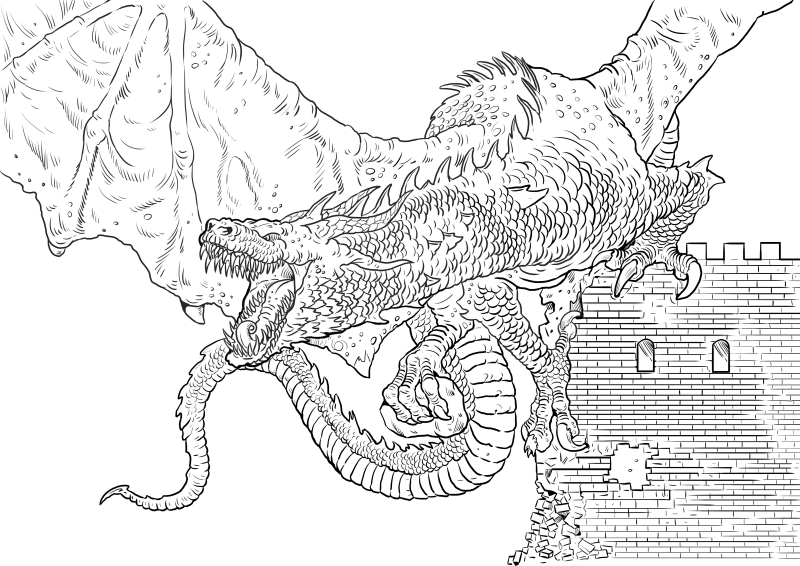
\includegraphics[scale=.5]{monsters/Dragon2}
\end{center}

\begin{multicols*}{2}

\myhighlight{Breath Weapon}{dragon-breath-weapon}

  \mytable{c c c X}{
    \thead{\SUM Age+Size} & \thead{Damage} & \thead{Uses} & \\
  }{
    2-4 & 6d6 & 1 & \\
    5-7 & 7d6 & 1 & \\
    8-10 & 8d6 & 2 & \\
    11 & 9d6 & 2 & \\  
    12 & 10d6 & 3 & \\
  }

Note that a dragon's breath weapon affects all Close OR Nearby (Distinct) Adventurers, and hits automatically. 

There are 2 ways to reduce the damage from a breath weapon:
\mybullet {
  \item Make a \RSTRY{\TAL}. If you don't roll a Failure, take half damage.
  \item Make a \SAVE{Doom}. If you succeed, take half damage again.
}

These effects stack - so making your \RS:\TAL try and a \SAVE{Doom} will reduce the amount of damage by 75\%. Roll the check and Save before you apply damage.

The color of the dragon also affects the breath weapon type:


\vspace*{8mm}

\mybold{Red:}   Fire.  \RS:\TAL. If you fail, you become \mylink{Enflamed}{effect-enflamed}.

\mybold{Black:}  Acid.  If the attack hits Flesh, take 2d4 acid damage for 2d4 Moments.

\mybold{White:} Frost. \SAVE{Doom} or take \DCDOWN damage to a single facet of your \mylink{Identity}{adventurer-identity} (your choice).

\mybold{Blue:}  Lightning.  If you're wearing metal armor, take an additional 2 points of damage per die.

\mybold{Green:}  Corrosive gas.  Everyone must try their Armor \UD 3 times.

\mybold{Bone:}  Void.  \SAVE{Doom} or take \DCDOWN damage to a single facet of your \mylink{Personality}{adventurer-personality} (your choice).

\mybold{You can sunder your shield to prevent the secondary effect (but not the damage).}

  \newpage

}
